% !TeX program = xelatex
\documentclass[UTF8,11pt,fontset=windows]{ctexart}
\usepackage[a4paper,left=22mm,right=22mm,top=21mm,bottom=21mm]{geometry}
\usepackage{fontspec}
\setmainfont{Times New Roman}
\setsansfont{Arial}
\usepackage{array,booktabs,longtable,tabularx}
\usepackage{xcolor}
\usepackage{enumitem}
\usepackage{amsmath}
\usepackage{graphicx}
\usepackage{fancyhdr}
\usepackage{pdflscape}
\usepackage{needspace}
\usepackage{hyperref}
\hypersetup{colorlinks=true,linkcolor=black,citecolor=black,urlcolor=blue!45!black,pdftitle={老旧小区更新辅助决策技术说明：模式研判、投资比较与收益评价},pdfauthor={朱航成}}
\renewcommand{\arraystretch}{1.28}
\setlength{\tabcolsep}{4pt}
\setlength{\parskip}{3pt}
\linespread{1.22}
\setlist[itemize]{leftmargin=1.8em,itemsep=2pt,topsep=4pt}
\setlist[enumerate]{leftmargin=2em,itemsep=3pt,topsep=4pt}
\ctexset{section={format=\large\bfseries,beforeskip=12pt,afterskip=6pt},subsection={format=\normalsize\bfseries,beforeskip=8pt,afterskip=4pt},subsubsection={format=\normalsize\bfseries,beforeskip=7pt,afterskip=3pt}}
\pagestyle{fancy}
\fancyhf{}
\fancyfoot[C]{\small\thepage}
\renewcommand{\headrulewidth}{0pt}
\renewcommand{\footrulewidth}{0pt}
\setlength{\headheight}{14pt}
\raggedbottom
\clubpenalty=10000
\widowpenalty=10000
\emergencystretch=2em
\newcolumntype{L}[1]{>{\raggedright\arraybackslash}p{#1}}
\newcommand{\field}[2]{\par\noindent\textbf{#1}\quad #2\par}
\newcommand{\decision}[2]{\Needspace{7\baselineskip}\subsection*{#1\quad #2}}

\title{\bfseries\Large 老旧小区更新辅助决策技术说明\\模式研判、投资比较与收益评价}
\author{\normalsize 建工 AI 项目\quad 朱航成}
\date{\small 2026年10月15日}

\begin{document}
\maketitle
\vspace{-6mm}

本工作台面向老旧小区更新的前期辅助决策，回答三个问题：\textbf{片区要不要更新、值不值得投入、投入后产生哪些财务与社会收益。}真实项目先确认是否已有居民满意度、需求、鉴定及预算资料，有则导入当前项目后再由AI初判；随后比较综合整治与原拆原建条件，把方案、资金、受益对象和调查任务对应到原文，确定研究与实施的先后顺序。

核心成果是由AI综合研判、以证据标准约束的辅助决策方法：\textbf{模型负责解释、程序负责判定。}模型主动读取项目资料与对标案例，归纳关键矛盾、比较改造路线，提出更新方式、投入阶段及财务与社会收益的条件化决策，并给出理由和出处。程序核对来源、对象与实施条件，复算数值，保留模型建议和准入结果。方向判断页直接呈现真实API的综合研判；关键缺项落实为调查任务，六维权重供使用者比较侧重。造价正文采用分阶段、同口径参考区间，神经网络与模拟细节集中于附录。

\section{研究对象与需要回答的问题}

求是村位于杭州市西湖区灵隐街道浙大求是社区内，邻近浙江大学玉泉校区。现有材料涉及二次供水、加装电梯及后续托管、邻里中心服务等不同事项。研究将社区、住宅区、楼幢、单元、设施及服务路线作为不同对象层级，分别建立档案。

用户选中区域并确认本项目可用材料后，取得首轮方案方向及依据，再按下表评估投入与收益。居民日常困难、维修或拆建条件、资金和维护安排共同决定下一步行动。

\begin{longtable}{@{}L{31mm}L{67mm}L{61mm}@{}}
\toprule\textbf{决策问题}&\textbf{重点比较}&\textbf{交付给使用者的内容}\\\midrule
要不要更新&安全与使用问题、居民需求、可修复性、权属规划与协商安置&模式初判、已有依据、阻断条件及专项调查顺序。\\
值不值得投入&同范围建设与安置成本、资金落实、收入权利、运营支出及现金缺口&分阶段同口径造价参考、方案资金表、财务收益与敏感性。\\
投入带来什么&去重受益人数、服务可达与利用、未满足需求、维护和居民影响&财务收益与社会收益分账、现况与改后目标对照、后续观测计划。\\
\bottomrule\end{longtable}

产品最终交付的内容包括项目总体建议、逐项改造建议、建议理由、原文证据、适用规则、备选方案、资金表和调查任务。每项建议围绕一个明确对象展开，形成“对象与问题、行动、理由、规则、来源、下一步”的完整记录。

\subsection{核心判断标准：证据、条件与偏好分层}

四层标准连接项目证据、实施条件、数值核算与决策偏好。模型主动综合需求、工程、协商和资金材料，识别关键矛盾并比较路线，提出条件化决策及理由。程序按适用文件的版本、条件和出处核验建议，执行来源与实施准入检查；偏好由使用者调整。模型研判与程序结果分别保存，供复核建议的形成依据与推进条件。

\begin{longtable}{@{}L{29mm}L{70mm}L{60mm}@{}}
\toprule\textbf{判断层}&\textbf{采用的标准与证据}&\textbf{程序形成的结果}\\\midrule
\endfirsthead
\toprule\textbf{判断层}&\textbf{采用的标准与证据}&\textbf{程序形成的结果}\\\midrule
\endhead
证据准入&原件、对象、版本、定位、形成日期与工程阶段对应；当前事实、历史事件和对标案例分别登记。&保留可引用片段；确认条件记为满足或不满足，缺项及分歧记为未知或冲突。\\
模式与行动准入&逐栋修缮可行性、拆除与保护、权属规划、居民决议、安置、资金、全周期比选和维护责任。&逐项显示触发条件；形成优先研究路径、指定调查或暂缓事项。\\
投资与收益核算&同范围工程量与价格阶段；已落实出资；有权实现的销售、出租及服务收入；受益人数、服务量及各自分母。&分列建设与安置成本、资金缺口、财务现金流和社会收益，再做敏感性比较。\\
六维偏好比较&居民需求、公共服务、居住工程、实施协同、长效维护、资金交付的评价与用户权重。&显示各维贡献、已评估权重比例与可能分值范围；偏好变化更新比较结果。\\
\bottomrule\end{longtable}

模式初筛以保留建筑、综合整治作为研究基线。当前拆建准入登记九项条件：\textbf{结构修缮不可行、拆除与保护允许、权属边界明确、重建规划确认、居民决议有效、腾退回搬落实、项目资金落实、全周期方案已比选、维护责任明确。}九项均有对应对象的有效证据时，具备原拆原建优先前期论证所需条件；修缮不可行而拆建条件待补时，优先安排安全和实施条件专项核查。该规则是本工作台的前期研究准入，具体专业认定和法定程序由对应文件确定。功能重构或经济必要性的其他拆建理由进入专项论证，补充其适用条件与证据后再判断。

正式行动另按证据完整性和适用规则区分“建议开展专项调查”“先补充关键资料再判断”“当前条件下暂缓”。偏好比较在这一边界内说明方案取舍，安全、权属与程序条件持续单列。

\subsection{求是村实例：一条原文怎样改变判断}

\begin{longtable}{@{}L{27mm}L{132mm}@{}}
\toprule\textbf{判断环节}&\textbf{供水举措的具体处理}\\\midrule
\endfirsthead
\toprule\textbf{判断环节}&\textbf{供水举措的具体处理}\\\midrule
\endhead
标准&楼幢、批次和阶段对应，按施工、验收、接管及运行资料认定进度。\\
证据&2023年8月18日原文：29、30、31、48幢共252户拟改；留博楼因泵房位置未纳入。\cite{water}\\
条件&四幢核后续工程与运行档案，留博楼补独立技术路径；拆建条件逐栋另核。\\
结论&综合整治优先研究；四幢核阶段与接管，留博楼查泵房和系统衔接，拆建列条件备选。\\
权重与更新&提高服务偏好比较覆盖，提高资金偏好核分期及维护；新增原件更新对应条件和版本。\\
\bottomrule\end{longtable}

这条链将历史报道落实为两个不同对象的调查和技术任务。模型解释分路原因，程序保留252户的原范围与时点，并核验新资料是否改变条件；一项已有更新经验由此进入可执行的当前研究。

\subsection{可调权重怎样服务方案比较}

使用者在0至5范围设置六维权重，至少一项为正；程序归一化为$w_d\geq0$且$\sum_dw_d=1$。真实资料的低、中、高评价分别映射为1、3、5级，展示标尺为20、60、100。已评估维度须具有唯一的维度记录，且引用可对应本次方案包来源；每维保留原文理由，待核维度保留空值。设$K$为已评估维度，$C$为其权重合计，$B$为已知贡献，则
\[
C=\sum_{d\in K}w_d,\qquad B=\sum_{d\in K}w_d(20s_d),\qquad
S\in\bigl[B+20(1-C),\ B+100(1-C)\bigr].
\]
全部正权重维度已有评价时，范围收敛为单一偏好分值；存在缺项时，同时展示$B$、$C$与上下界。这里的范围由待核维度的完整展示刻度推导，表达资料缺口对比较的影响。范围交叠的方案并列比较其关键差异，补充能改变取舍的证据后再确定顺序。

滑杆表达“该项从低到高改善的价值”，同时考虑表现差距与决策者对这一改善的重视程度。英国政府多准则分析手册及经济方案比较指导采用这种摆幅赋权思路，要求解释权重和方案取舍，并检验权重变化的影响。\cite{mca2009,mcda2024}本项目据此实现同一低、中、高适配标尺下的\textbf{目标偏好敏感性}；预设提供可编辑的讨论起点，等级、改善价值与权重由具体项目的专业复核逐步校准。

审批沟通可对照“综合平衡”“居民改善优先”“财政承受优先”三组可编辑设定，说明同一方案在哪些目标上更有优势，并与建设资金表、财务现金流、去重受益人数及未满足需求对照。权重只改变比较侧重；模式准入、费用公式、原文与事实保持各自的核验结果。对应计算入口为\path{packages/retrofit/decision-priorities.ts}。

\subsection{价值如何验证}

评测采用同资料、同问题、同交付要求的对照。验证计划分别考察资料定位时间、引用与阶段核对正确性、方案遗漏和调查任务可执行性；按项目保留原始计时、答案清单与错误记录。下表把技术能力与实际决策价值对应起来。
\begin{longtable}{@{}L{33mm}L{70mm}L{56mm}@{}}
\toprule\textbf{评价方面}&\textbf{对照方法}&\textbf{记录指标}\\\midrule
资料初核效率&相同材料与问题，比较逐份阅读核对和工作台定位&总耗时、引用查找次数、完整交付比例。\\
证据与结论质量&由专业人员对照原件，复核对象、范围、日期、阶段和连续引文&引用正确性、关键遗漏、冲突识别、需人工修正的事项。\\
方案与收益比较&固定对象及资金口径，分别变更举措范围与目标偏好，复算费用并记录取舍&资金缺口、财务现金流、去重覆盖与未满足需求；硬条件独立核对。\\
调查落地&检查每项待核问题能否落实到对象、持有人和所需文件&任务可执行性、完成后可重算的判断及版本变化。\\
\bottomrule\end{longtable}
\subsection{公开工作台四主题资料初核自测}
2026年10月15日，在校园服务器求是村资料v14的78条来源登记、2份解析文档上，固定供水、电梯、社区康养和停车对标四个问题、12 项核对标准。服务已运行、资料已解析且未清缓存的单批次中，四请求并发定位耗时0.388 秒；加上原文逐字核对、版本检查和资料快照复查，自动流程耗时0.494 秒，前五条结果支持12/12 项核对，返回的17/17 条片段可回到当前资料版本。

相同问题与资料快照的前测为8/12 项，本轮为12/12 项，前后原始记录及遗漏项保留在附录。 该数值为自动流程自测；人工配对评测按上表执行。


\section{已有调研、真实数据与历史造价参考}

本项目已围绕求是村供水、电梯托管、加梯公示和邻里中心查阅公开原文，并沿浙江、上海、广东公共资源交易及住宅修缮平台收集历史改造工程。资料形成两层数据：一层为已归档、能逐字段回读的官方原件；另一层为AI辅助采集并保留来源地址的扩展工作簿，继续按原件补核。网上采集、字段计算与原文核验分别登记。

\begin{longtable}{@{}L{37mm}L{63mm}L{59mm}@{}}
\toprule\textbf{资料层}&\textbf{现有规模}&\textbf{在决策中的用途}\\\midrule
\endfirsthead
\toprule\textbf{资料层}&\textbf{现有规模}&\textbf{在决策中的用途}\\\midrule
\endhead
官方工程原件&27份归档原件，20条价格阶段记录&核对金额、范围、面积和价格年，形成有出处的参考组。\\
浙沪粤扩展工程库&1277条工程行：浙江1181、上海50、广东46&扩大案例发现范围，按项目及标段联结公告，逐项完善工程口径。\\
扩展库金额字段&预算694、控制价194、中标831、合同1146、结算0条&同一工程可有多个阶段字段；分别保存，不将字段数相加作为项目数。\\
案例与规则基线&23条案例及规则记录，保留原卡号；另有27条筛选规则&把历史举措、条件和出处对应到当前方案与调查任务。\\
杭州公共服务问卷&已读取公开原附件2236份、38个小区、84个字段&审计量表及社区群集结构，为调查设计和服务比较提供依据。\\
\bottomrule\end{longtable}

扩展库来自2026年10月14日补全工作簿，保留原表、单元格定位、来源地址及提供方核验说明，1277行按待复核扩展工程记录使用；已完成逐字段原文核对的记录进入归档层。案例规则基线沿用2026年10月12日快照，其中求是村15条、公开案例与规则库7条、翠苑历史资料1条。\hyperlink{EXP-16120dfe-9d94-4394-8880-494b385cf2d2}{C01}至\hyperlink{EXP-1d56715f-f6b6-4e9f-8298-5ce656ee40c5}{C23}对应原卡号，D0至D12对应后文的具体决定。

\subsection{正文采用的造价结论：分阶段同口径库＋参考区间}

前期投资判断采用带来源的工程量、单价和历史参考组。工程先区分施工、EPC及其他费用范围，再分别登记估算、预算、控制价、中标、合同与结算；金额与面积必须属于同一工程或完整标段，按地区、年份与面积含义形成参考区间。参考组显示样本数、最小值、中位数和最大值，并列出排除原因，供方案预算与进一步询价使用。

造价正文使用可回查的同口径参考区间。附录\ref{app:cost-neural}另保留神经网络辅助探索的原理、中标数据试验、七指标合成示例及中位数和岭回归对照，分别说明其数据范围与实验结果。

\section{改造模式前置与经济可持续性}

模式判定采用七个可组合的物理家族，另行登记组织、资金、工程交付和运营方式。自主更新是组织与出资机制，EPC是交付方式；它们可与保留修缮、局部拆建或整体重建共同出现。比较单位为同范围、同目标且包含工程、安置、经营与维护的方案包。\cite{renewal2025,hzmode}

\begin{longtable}{@{}L{16mm}L{44mm}L{99mm}@{}}
\toprule
\textbf{模式} & \textbf{物理方式} & \textbf{候选条件与可组合措施}\\\midrule\endfirsthead
\toprule\textbf{模式} & \textbf{物理方式} & \textbf{候选条件与可组合措施}\\\midrule\endhead
M01 & 保留综合整治 & 现有建筑具备继续使用条件，主要问题集中于管线、公共部位、环境与设施；管线更新、屋面外墙维修、无障碍、停车充电。\\
M02 & 结构加固与专项修缮 & 专业鉴定和工程论证明确加固或修缮路径及价值；抗震加固、构件修缮、防水、节能。\\
M03 & 成套化与适度改扩建 & 厨卫、户型或交通功能短缺，结构、空间和规划审批允许改善；独立厨卫、户型调整、住宅扩面、加装电梯。\\
M04 & 局部拆建与保留 & 安全、功能及土地条件差异集中于特定楼栋或分区，能够建立分区审批和过渡安排；逐栋处置、保留加固、局部新建、分期安置。\\
M05 & 整体拆除重建 & 范围内住房质量和功能问题广泛，并明确拆建审查、规划、产权、居民协商与安置路径；拆除、住宅重建、回迁、公共服务。\\
M06 & 保护性修缮与适应性利用 & 纳入保护名录或保护控制范围，允许的修缮与利用方案经对应程序确认；保护修缮、设施改善、允许的用途适配、容量控制。\\
M07 & 功能置换与服务设施植入 & 存量空间权利、允许用途及服务需求可衔接，消防、服务容量和运营安排明确；闲置房改用、邻里中心、养老托育、便民商业。\\
\bottomrule\end{longtable}

方案生成先识别逐栋鉴定与适修性、保护和权属、规划与面积用途、居民意愿及安置。通过这些条件后，对可组合措施比较资金、市场、支付能力、维护和居民效果。缺项影响对应方式；其他具有明确条件的方案继续研究。

研究框架采用\textbf{前置模式判定＋原六维＋市场收益维度}。市场收益同时记录售价、租金、客群、可支付预算、可处置面积和收益归属，使方案比较既回答投入，也回答收入与长期维护如何衔接。

\subsection{按收款人和受益人建立四本账}

\begin{itemize}
\item 成本账：工程、过渡安置、设计检测、迁改、运维和交付。
\item 现金收入账：具有对应使用与处分或收费权利的对外销售、出租和服务收入，保存收款主体、时点及价格口径。
\item 资金安排账：居民、产权单位及财政出资，贷款和还本息；分别核对计划与已落实时序。
\item 资产与公共效益账：业主住房价值变化、便利改善、设施覆盖和使用效果，保存受益对象及评价方法。
\end{itemize}

新增面积分成原住户回迁、自选扩面、安置及保障住房、公共服务和获准市场处置。每类记录面积、用途、权属及收款主体。浙工新村的居民扩面付款与产权人二手售房分别登记；上海案例的厨卫改善面积与增量房源政策也按用途分列。\cite{zhegongdata,shmix}

\subsection{用同一基线说明投入换来什么}

“值不值得投”落实为候选方案相对维持现状或最低必要维修的增量比较。财务侧登记新增建设、安置及运维支出，以及项目主体有权取得的收费、租金和处置收入，比较净现值、资金峰值和居民负担；社会侧登记新增去重受益人数、连续可达人数、服务利用、尚未满足需求和施工期影响。每项变化均保留对象范围、月份或评估期与数据依据。

例如，增加一段无障碍路线时，程序对应增加的工程量和维护费用，模型说明该路线连接哪些居民与服务设施，覆盖计算再给出新增可达及使用人数。政府支付作为财政成本进入资金账，运营方收取的购买服务或补贴进入其现金账；出行便利与居民受益在社会效果中列示。由此能说明“更新哪一部分、增加多少投入、谁取得现金、哪些居民获得改善”，供使用者比较实施范围与次序。

\section{材料如何拆分并沉淀}

\subsection{先建立材料与对象之间的关系}

资料按内容和用途分组。项目原件用于记录对象与工程阶段，政策文件用于建立程序和专业条件，案例与论文用于整理可比较因素及措施选择的方法。每份材料登记名称、发布或形成日期、提供主体、空间范围、资料类型、原件版本和对应对象。

\begin{longtable}{@{}L{28mm}L{72mm}L{59mm}@{}}
\toprule
\textbf{材料类型} & \textbf{重点读取的内容} & \textbf{形成的记录}\\
\midrule
\endfirsthead
\toprule
\textbf{材料类型} & \textbf{重点读取的内容} & \textbf{形成的记录}\\
\midrule
\endhead
对象与工程档案 & 楼幢单元清册、图纸、面积、设施位置、检测、设计、施工、验收与移交。 & 对象档案、工程问题、措施范围和阶段链。\\
居民调查与协商 & 受访对象、需求、使用困难、支持与异议、费用承担及方案回应。 & 分群需求、协商事项、受益与影响对象。\\
预算合同与运维 & 工程量、单价、费用项目、出资状态、支付节点、服务边界和运行工单。 & 分项投入、资金接口、维护责任与表现。\\
公开项目材料 & 项目公示、进展报道、启用记录、具体举措、参与主体和报道时点。 & 带时点的历史事件、调查入口和案例线索。\\
政策与专业文件 & 改造类别、实施程序、专业前置条件、资金与建管要求、适用范围。 & 条件规则、核查项目与条文出处。\\
历史案例与论文 & 措施选择、关键因素、比较方法、组织过程、执行结果和适用条件。 & 经验卡、候选因素、规则复核材料。\\
\bottomrule
\end{longtable}

\subsection{围绕动作形成可以引用的片段}

切分先识别“在哪个对象上采取了什么动作”。电梯加装、水泵更新、管道修复、坡道设置、物业托管和服务时段调整分别成为举措条目。对象、动作或实施阶段发生变化时建立新条目；同一举措在多段文字、表格或附件中出现时，通过原文位置连接。

原文层保留标题、段落、页码、表头、行列和单位。举措层将对象、现状问题、条件、投入、实施过程、结果及维护联系起来。检索时先找到相关举措，再展开其上级工程背景和关联原文，使面积、金额、单位及例外条件保持完整。

例如，一份报告的正文介绍电梯安装，表格列出费用，附件记录居民意见。知识库将三个位置关联到同一项电梯举措：正文对应措施，表格对应投入，附件对应实施协同。整体工程金额保存在工程层，有明确分项的投入再对应到具体措施。

\subsection{每张经验卡保存什么}

一张经验卡按以下字段组织：所属项目与楼幢单元、决策问题、对象背景、具体举措、关键条件、备选措施、实际决定、选择依据、实施过程、运行结果、维护责任及迁移条件。每个字段关联原文位置和版本，提议、决策、施工、投用和运行分别保存阶段记录。

面积分为土地面积、建筑面积和实际改造面积；人数分为住户、居民、受益对象和受访者；费用分为建设预算、合同、支付、运行维护及大修。新取得的合同、检测或复盘资料追加到对应举措，形成可查询的版本链。

\subsection{求是村二次供水改造的拆分实例}

\field{已有案例卡}{\hyperlink{EXP-8fb43037-0680-4136-8844-edcb789391f4}{C14}保存29、30、31、48幢及252户因素；\hyperlink{EXP-89d54bcc-fc1f-4431-be62-7a06bce77e41}{C12}保存踏勘与方案外审的提议字段；\hyperlink{EXP-16120dfe-9d94-4394-8880-494b385cf2d2}{C01}关联进场计划及留博楼泵房位置，其他供水卡关联同文背景。}

2023年8月报道记载，拟改范围为29、30、31、48幢，共252户。现场踏勘发现水表老旧、部分管道锈蚀渗漏和泵房布局紧凑等问题，方案涉及水泵设备更新及参数优化、水池和管道材质提升、水表改造。留博楼因当时泵房位置问题单列。\cite{water}

\begin{longtable}{@{}L{35mm}L{124mm}@{}}
\toprule
\textbf{记录层级} & \textbf{本例怎样填写}\\
\midrule
\endfirsthead
\toprule
\textbf{记录层级} & \textbf{本例怎样填写}\\
\midrule
\endhead
工程父级 & 求是村该批次二次供水改造；范围29、30、31、48幢；252户；资料时点2023年8月。\\
举措条目 & 水泵更新与参数优化、管道材质提升、水表改造分别关联到该工程。\\
问题与条件 & 水表现状、管道锈蚀渗漏、泵房空间、现有直供与加压方式、设计及外审材料。\\
阶段记录 & 现场踏勘、方案外审、公示、合同签订及进场准备，按报道记载逐项保存。\\
特殊对象 & 留博楼的泵房位置及后续技术方案，建立单独对象和问题记录。\\
后续材料 & 施工及变更、验收、接管、运行工单、压力观测和检测资料，继续关联到具体楼幢与设施。\\
\bottomrule
\end{longtable}

\field{六维对应}{楼幢、系统和泵房进入居住工程；踏勘与外审参与主体进入实施协同；接管和运行资料进入长效维护；工程量及费用进入资金交付。}
\field{规则与决策对应}{已有基础类规则卡\hyperlink{EXP-e1688c4c-a449-48d4-9d16-38fea3ca845e}{C22}形成R2，长效管理卡\hyperlink{EXP-6baff473-93ed-4160-9a93-a0abf3c7b092}{C19}形成R3。由本案例形成D4逐幢供水调查，并由留博楼的特殊条件形成D5独立技术子题。}

\subsection{电梯托管与邻里中心的拆分实例}

\textbf{电梯托管。}库中\hyperlink{EXP-1f50f306-64e5-4335-be56-5c89531c00f2}{C03}已经保存决策问题“维护和保养怎么解决”、多方协商的实际决定及居民反馈；\hyperlink{EXP-3092f687-50c6-452e-b1d1-5703c250c25e}{C07}保存托管费用、协议和管理细则的条件字段。2023年12月原文记载费用从600元降至300元/台/月。\cite{trust} 对应关系为：协商主体进入实施协同，服务职责进入长效维护，费用进入资金交付。R1居民参与来自\hyperlink{EXP-c48118fa-9af5-4f9a-a634-ae276701cc6a}{C21}，R3长效管理来自\hyperlink{EXP-6baff473-93ed-4160-9a93-a0abf3c7b092}{C19}；据此形成D2托管后评估、D3单元协商及D10建设维护费用表。年化托管额按300元/台/月折算为3600元/台。

\textbf{邻里中心。}\hyperlink{EXP-8ab942a8-bdac-4075-97da-46b09ee9aa41}{C13}已有启用背景及公共服务描述；关联的2025年10月原文包含康养、文化、儿童与家庭服务。\cite{neighbor} 这张卡对应居民需求和公共服务，继续连接服务主体、开放时段和运行反馈。\hyperlink{EXP-2c88cc20-e2d3-4a32-a176-e48d753a4712}{C16}的AIPA规则入口形成R4，帮助教师选择需求和优先级调查因素；\hyperlink{EXP-6baff473-93ed-4160-9a93-a0abf3c7b092}{C19}形成R3，连接服务运行安排。最终对应D6居民到达路线及D7邻里中心服务组织比较。

\subsection{跨项目案例与论文怎样进入知识库}

库中的翠苑资料已经拆出\hyperlink{EXP-4fb5ae8b-4f8c-4b38-9f15-7fd612098a66}{C17}道路、\hyperlink{EXP-54fdb799-7504-45fd-bd7a-b619e98cf6cb}{C18}外墙面和\hyperlink{EXP-825f931a-a8d3-49c2-9c42-e73bea9922e6}{C20}绿化景观三张卡，\hyperlink{EXP-1d56715f-f6b6-4e9f-8298-5ce656ee40c5}{C23}另保存54栋住宅楼和8幢公建的历史实施范围。三项举措共享2022年工程原文，其中记录3110户，以及沟通协调、工序优化和现场组织。\cite{cuiyuan}

\textbf{\hyperlink{EXP-4fb5ae8b-4f8c-4b38-9f15-7fd612098a66}{C17}道路。}已有实施字段关联道路整治、验收和现场组织。居住工程记录路段与工程内容，实施协同记录工序及住户沟通。结合R2基础设施和R1居民参与，求是村可按实际路段开展D6路径观察、D8空间使用比较及D9分期接口分析，调查中补充路面、排水、通行与施工占用。

\textbf{\hyperlink{EXP-54fdb799-7504-45fd-bd7a-b619e98cf6cb}{C18}外墙面。}已有实施字段关联外墙整治和该工程实施背景。居住工程继续记录具体楼幢、检查问题与施工范围，资金交付记录工程量和费用。求是村对应D1楼幢问题清册及D9综合工程包比较；专业检查确定维修、防水或表面整治的具体内容。

\textbf{\hyperlink{EXP-825f931a-a8d3-49c2-9c42-e73bea9922e6}{C20}绿化景观。}已有实施字段关联绿化改善及共同工程过程。居民需求和公共服务关注休憩与活动使用，居住工程关注位置、道路和设施接口，长效维护关注养护职责。结合R1、R3和R4，求是村对应D6适老路线及D8公共空间比较，调查中补充实际使用、遮阴、照明和养护事项。

库中\hyperlink{EXP-2c88cc20-e2d3-4a32-a176-e48d753a4712}{C16}的决策依据字段指向AIPA矩阵结果，关联的西安居民满意度研究将区位、基础设施、交通、居住管理和生活设施作为调查属性，利用非对称影响分析研究改造优先顺序。\cite{paper} 教师可从这张规则入口及原文中挑选适合求是村的调查因素，形成R4，再用于D6、D7及措施排序。

\section{用户数据表与逐行采集规则}

字段体系以三份已有表格为依据：46项核心指标、27条筛选规则、76项默认缺省扩展字段和15项专家待补。全部原编号、原值、年份、空间口径、原说明及单元格定位保留。来源分为公开、问卷与访谈；尚未采集的字段登记为缺项。案例卡C01、数据字段C01和模式M01使用不同命名空间，正文分别写“案例”“数据”“模式”。

核心表S02至S16的15项演示值保持原来的模拟标签；B、D、M、C中的空项保留空值。规范条目沿用用户筛选；专家意见在E01至E15上补充。已有经验规则R1至R4与用户规范规则R001至R027分别引用。



\subsection{默认缺省字段按报告需要补填}

76项扩展字段默认值为缺省，初次运行以核心指标和已有材料组织报告。扩展字段覆盖道路排水、无障碍、公共服务、设计消防及加梯产权，按原表关联到具体规则。

当报告采用某条规则，且该扩展字段会改变所建议的措施或理由时，生成补填任务。任务保存字段ID、规则ID、影响哪项建议、向谁查询、怎样采集、原表位置和补齐后重算什么。补齐只更新相关规则与方案版本，其余任务继续运行。

例如，报告提出连续无障碍路线并引用R007，便按需请求X013路径与X014断点，其余74项保持缺省。人工补填X013后，该项进入复核，X014仍待补；道路评级引用R001时，请求对应病害台账。选择性收益缺项时，基线先不计这部分加成；若某项收入已经承担资金平衡或运维覆盖任务，则将它列为该方案的关键补充项。

\subsection{内部文件与互联网调查怎样相互补充}

初判前先询问是否有本项目的居民满意度、需求、鉴定或预算材料，并将已有文件导入当前项目。内部文件解析保留楼栋清册、分群人口、设施合同、费用和使用台账；问卷访谈补支付上限、出行困难与服务体验，互联网调查补政策、进度和市场样本。材料保存项目范围、来源类别及原文位置，上传时间与声明的材料日期分列，未知日期保留为空；每轮明确选择内部材料是否参与模型分析。这里的内部资料是项目来源类别，校园协作采用共享访问范围。

老年人数采用同一研究范围的脱敏人口汇总；覆盖率采用目标群体和去重服务对象；应用情况同时保存使用人数、访问次数、设施容量和观察月份。已保存的历史社区人口与当前小区台账分别记录，供背景、参数参考和实际核算各自使用。

\begin{landscape}
\small
\begin{longtable}{@{}L{21mm}L{55mm}L{50mm}L{34mm}L{45mm}L{32mm}@{}}
\toprule
\textbf{维度与原ID} & \textbf{数据内容} & \textbf{对应判断} & \textbf{来源与缺项} & \textbf{采集方式} & \textbf{规则对应}\\\midrule\endfirsthead
\toprule\textbf{维度与原ID} & \textbf{数据内容} & \textbf{对应判断} & \textbf{来源与缺项} & \textbf{采集方式} & \textbf{规则对应}\\\midrule\endhead
前置模式判定
\newline B01、B04、B09等 & 逐栋适修性、权属与保护、规划容量、居民协商、面积用途和过渡安排。 & 生成保留、加固、改扩建、局部拆建、整体重建与服务组合。 & 公开＋访谈；鉴定、许可及分户权利待采 & 官方目录、获准原件解析、测绘、规划与产权方访谈 & MODE-G01至G04\\
居民需求
\newline B05、B06、B07等 & 常住及老年人数、行动困难、现住与目标客群、预算、需求和意见。 & 确定服务对象、居民分摊与支付匹配，选择适老改善顺序。 & 公开＋问卷＋访谈；实际住户预算缺项 & 脱敏台账、分群问卷、访谈；历史人口按原范围引用 & R007；ECON-AFFORD\\
公共服务
\newline D06、S04、S08等 & 设施位置、对象、开放与容量、价格、连续可达、实际使用和覆盖。 & 比较已有中心、共享设施、路线与时段调整及服务植入。 & 公开＋问卷＋访谈；使用记录待采 & 目录与合同解析、服务路线、台账和去重使用调查 & R008至R013；R007\\
居住工程
\newline B02、B03、D01等 & 楼栋、设施、鉴定、道路管网、厨卫与电梯、可改和拆建范围。 & 按栋生成措施，区分供水、加梯、成套化、修缮及拆建接口。 & 公开＋访谈；专业原件待取得 & 图纸、检测、公示和验收解析；现场点位核查 & R001至R007；R014至R024\\
实施协同
\newline B01、B09、S13等 & 主体、权利、协商、安置、施工扰动、过渡期及分期衔接。 & 区分自主组织、代理建设和工程方式，形成责任与安置表。 & 问卷＋访谈＋公开；法定记录待采 & 按事项台账、协议原件、各主体访谈 & MODE-G04；R021至R024\\
长效维护
\newline S15、S16 & 接收方、运维服务、合同、年度支出、维护覆盖与交接。 & 核谁维护、谁收费、经营净额能覆盖多少持续支出。 & 公开＋访谈；经营与维保合同待采 & 合同条款抽取、费用和工单核对、运营方访谈 & MODE-G06；ECON-MAINTENANCE\\
资金交付
\newline B10、C01、C02等 & 建设、安置、运维、出资、补助、借款本息、到位与结算。 & 比较年度现金缺口、居民负担和融资时序，确定方案包。 & 公开＋访谈；本项目报价与出资待采 & 工程量与报价、资金原件和支付计划解析 & R025至R027；ECON-COST；ECON-FUNDING\\
市场收益
\newline M01、M02、M03等 & 同类交易与挂牌、租金、吸纳、面积用途、经营权、费用与客群预算。 & 计算可实现销售、出租、服务现金；单列业主资产变化与公共效果。 & 公开＋问卷＋访谈；真实租约及处分权待采 & 同口径市场样本、租约和运营合同、预算问卷 & ECON-REALIZABLE；ECON-NPV；MODE-G05\\
\bottomrule\end{longtable}
\normalsize
\end{landscape}

\section{已有规则卡怎样参与专家判断}

\subsection{逐张规则卡对应到案例和措施}

现有公开资料库已经保存四张规则卡。下面按原卡解释其内容和求是村的使用位置，R1至R4是本文的讲述编号。教师复核时，在这些已有条目上确认适用场景、必要条件、比较因素和参数，并保存对应原文位置。

\begin{longtable}{@{}L{12mm}L{37mm}L{64mm}L{40mm}@{}}
\toprule
\textbf{规则} & \textbf{原卡与依据} & \textbf{怎样转为判断条件} & \textbf{案例与决定}\\
\midrule
\endfirsthead
\toprule
\textbf{规则} & \textbf{原卡与依据} & \textbf{怎样转为判断条件} & \textbf{案例与决定}\\
\midrule
\endhead
R1 & \hyperlink{EXP-c48118fa-9af5-4f9a-a634-ae276701cc6a}{C21}居民自愿；政策原文。 & 明确具体事项的参与主体、需求、受益和影响，保存协商过程与方案回应；教师确认调查和协商的组织尺度。 & \hyperlink{EXP-1f50f306-64e5-4335-be56-5c89531c00f2}{C03}托管协商、\hyperlink{EXP-8ab942a8-bdac-4075-97da-46b09ee9aa41}{C13}服务对象、翠苑沟通；D3、D6、D7、D9。\\
R2 & \hyperlink{EXP-e1688c4c-a449-48d4-9d16-38fea3ca845e}{C22}基础类；政策中的改造内容。 & 把供水、道路及相关基础设施问题对应到措施；结合检测、工程位置与接口选择处理方式。教师确认轻重缓急和专业前置条件。 & \hyperlink{EXP-8fb43037-0680-4136-8844-edcb789391f4}{C14}四幢供水、\hyperlink{EXP-16120dfe-9d94-4394-8880-494b385cf2d2}{C01}泵房、\hyperlink{EXP-4fb5ae8b-4f8c-4b38-9f15-7fd612098a66}{C17}道路；D4、D5、D8、D9。\\
R3 & \hyperlink{EXP-6baff473-93ed-4160-9a93-a0abf3c7b092}{C19}长效管理；建管衔接原文。 & 设施措施同时确定接收、服务责任、维护费用、故障与交接。教师确认维护条件怎样影响方案选择。 & \hyperlink{EXP-1f50f306-64e5-4335-be56-5c89531c00f2}{C03}托管、\hyperlink{EXP-3092f687-50c6-452e-b1d1-5703c250c25e}{C07}费用、\hyperlink{EXP-8ab942a8-bdac-4075-97da-46b09ee9aa41}{C13}服务；D2、D4、D7、D10。\\
R4 & \hyperlink{EXP-2c88cc20-e2d3-4a32-a176-e48d753a4712}{C16} AIPA；论文矩阵与关联全文。 & 从居民需求与满意度因素研究优先顺序，确定本地调查项、群体差异和比较方法。教师确认因素、采集方法及分析参数。 & \hyperlink{EXP-8ab942a8-bdac-4075-97da-46b09ee9aa41}{C13}邻里服务、\hyperlink{EXP-4fb5ae8b-4f8c-4b38-9f15-7fd612098a66}{C17}道路、\hyperlink{EXP-825f931a-a8d3-49c2-9c42-e73bea9922e6}{C20}绿化；D6、D7、D8及措施排序。\\
\bottomrule
\end{longtable}

\textbf{R1的具体使用。}电梯托管卡\hyperlink{EXP-1f50f306-64e5-4335-be56-5c89531c00f2}{C03}记载多方协商，居民参与卡\hyperlink{EXP-c48118fa-9af5-4f9a-a634-ae276701cc6a}{C21}保存政策中的参与原则。两条记录对照后，求是村调查可按单元或具体服务事项登记参与者、意见、费用和方案回应，形成D3的协商与设计比较。\cite{trust,policy}

\textbf{R2的具体使用。}供水卡\hyperlink{EXP-8fb43037-0680-4136-8844-edcb789391f4}{C14}已有楼幢与户数，\hyperlink{EXP-16120dfe-9d94-4394-8880-494b385cf2d2}{C01}关联特殊泵房条件；基础类卡\hyperlink{EXP-e1688c4c-a449-48d4-9d16-38fea3ca845e}{C22}提供措施分类入口。教师把供水安全可靠、设施现状和工程适用条件落实到具体对象，形成D4与D5的不同调查路径。\cite{water,policy}

\textbf{R3的具体使用。}托管卡\hyperlink{EXP-1f50f306-64e5-4335-be56-5c89531c00f2}{C03}保存管理决定，\hyperlink{EXP-3092f687-50c6-452e-b1d1-5703c250c25e}{C07}保存费用与协议描述，长效管理卡\hyperlink{EXP-6baff473-93ed-4160-9a93-a0abf3c7b092}{C19}给出建管衔接依据。三者共同转成管理主体、服务内容、运行费用及责任交接的规则字段，形成D2和D10。\cite{trust,policy}

\textbf{R4的具体使用。}\hyperlink{EXP-2c88cc20-e2d3-4a32-a176-e48d753a4712}{C16}已保存AIPA方法入口。读取关联论文后，教师选择求是村的具体调查属性，将居民对出行、设施和服务的评价与现状共同用于措施排序，形成D6、D7的研究安排。\cite{paper}

\subsection{程序检查与教师补充的专业判准}

程序另执行三组检查：G1核对对象、来源、时间与阶段；G2检查方案的工程安全、实施权利与保护条件；G3核对工程量、单位、费用、资金状态和计算。进入专项调查前，现有程序核对居民需求、工程评审、服务缺口、实施协同、资金、维护以及规则七项确认，保存触发条件和证据。

教师可在四张规则入口上补充连续出行路径、服务覆盖、专业工程条件和分期接口等具体判准。例如，沿户门至服务入口记录路线断点；用开放时段、到达和容量判断服务调整；以泵房图和专业意见比较供水路径。每项专业判准连接对应案例、检查方法和参数。

项目行动分为开展专项调查、补齐指定资料和暂缓指定方案。规则卡负责说明适用条件，程序执行确认与计算，Agent解释多维条件怎样共同改变措施选择。前述九项模式条件决定拆建是否进入优先论证，七项行动确认负责当前方案的研究行动；六维权重用于比较取舍，三者分别保存触发结果。

\section{市场收益与措施效果的可计算模型}

\subsection{现金收入与经营净现值}

经济原型按任意模式ID和组件列表输入，按现金主体分别计算。量价、出租率和服务合同构成收入：
\[
R_t=A_{\mathrm{sale},t}p_t+A_{\mathrm{rent},t}\rho_t\,12u_t+R_{\mathrm{service},t}.
\]
其中面积对应有权实现的销售或出租范围，$p_t$为销售单价，$u_t$为月租单价，$\rho_t$为出租率。工程、安置与维护费用记为$C_t$。融资前经营净现值为
\[
NPV=\sum_{t=0}^{T}\frac{R_t-C_t}{(1+r)^t}.
\]
程序另计算静态收支、保本价格、目标人群月度及一次性支付匹配。资金安排以年为时间桶，按出资、借款与还本息时序计算累计余额，最低余额形成年度口径的峰值资金缺口。可研参考大纲将市场、商业模式、现金流、融资及可持续性分别组织，为本模型提供工作结构。\cite{ndrcfinance}

\subsection{适老设施覆盖与使用情景}

设施模型将群体人数、楼栋条件、连续路线、采用率和服务容量作为参数。按匿名人员ID去重，区分可达人数、使用人数和重复访问次数：
\[
\text{潜在覆盖率}=\frac{\text{可达目标人数}}{\text{目标总人数}},\qquad
\text{使用人群覆盖率}=\frac{\text{去重使用人数}}{\text{目标总人数}}.
\]
可达者采用率以可达人数为分母，容量使用率以同月份可用服务次数为分母。改善某条路线、增加可达设施或服务容量后，模型重新计算各群体的使用与覆盖。结果记为情景预测，输入保留来源与假设。

用户表数据S12给出40\%至70\%的覆盖目标，S16给出75\%至85\%的可达目标。数据S12登记户口径，人数模型登记目标人数口径；每个目标先匹配其对象和分母，再与模型结果对照，研究达到目标所需的设施与服务组合。

\subsection{有数据与有模型分别怎样推进}

先交付可运行的计算方法、字段体系和措施情景；得到真实人口、合同、问卷与市场样本后替换相应参数。可量化部分输出人数、覆盖、现金和预算结果；共享服务、出行便利及保护价值采用明确的对象、机制和调查指标说明。专家确认必要条件与比较偏好，Agent据此组织最终理由和候选方案。


\section{用可复核方法提高计算和结论的科学性}

方法落实为四类具体计算：按工程范围和价格阶段建立历史成本参考组；按服务时段核算有效容量；计算改变收支结论的阈值及参数组合；对真实问卷先审计量表和抽样单位，再给出描述统计。正文展开真实造价和问卷资料；容量、收支及参数压力测试的公式与示例见附录\ref{app:science}。

\subsection{原始数据先保留，再核对对象、阶段和分母}

最初取得的AI采集工作簿包含3张表，主表有7条丽水工程、19个字段和14个计算公式；后续扩展至正文所列的1277条补全库。初版原表逐字节保留；程序分别读取原始数值、公式与缓存结果，14个公式的独立重算均与缓存一致。随后再核实公告来源、金额阶段和面积含义，算术检查与事实核验分别记录。

例如，腾龙一期的正式中标金额为17333131元，92815平方米来自同一完整标段的招标规模；二者可以沿标段编号回查。最高投标限价18997007元及该面积还由公开招标正文同一原件支持。叶坦区块的7732717元在招标正文第9页明确勾选为最高投标限价，第3页给出53021平方米的改造范围。正文中的道路作业面积、总改造范围面积和总建筑面积分别登记。

东升南区有道路面积，却包含多种工程费用；金山新村只记载“总改造面积”，具体面积口径仍需补核；正达阳光城的多名候选人报出同一金额，程序保存一个候选报价记录。由此避免三种错误：把综合费用除成道路单价、把不同面积混作同一分母、把多个投标人当成多个独立改造工程。

\subsection{先形成同口径参考组，再计算金额强度}

GAO成本估算指南要求明确费用范围、单位、价格时期及归一化依据。\cite{gao2020} 本系统按省市、工程类型、工程范围、价格阶段、面积口径和价格年份分组；没有可靠价格指数时保留分年结果。候选报价独立于正式中标，EPC合同独立于施工合同，通信分项独立于整体修缮。

现有官方原件归档包含27份材料、20条价格阶段记录；其中24份原件被金额、范围或规模字段直接引用，包括广州3个施工合同和上海4个施工中标项目。广州案例的合同金额及总建筑面积来自同一公告；上海案例以明确项目编号和C01施工标段联结中标与招标原件。只有C01或只有相似名称时，不进行跨项目联结。

对已通过口径核验的记录，定义综合金额强度
\begin{equation}
 I_j=\frac{\text{该工程或标段金额（元）}}{\text{明确口径的对应面积（平方米）}}.
\end{equation}
该指标首先服务于同类项目的初步比价；具体施工深度和工程量清单仍在组内逐项比较。受益住宅总建筑面积对应的金额强度，与实际施工的屋面、道路或管线单价分别处理。

\begin{center}\small
\begin{tabular}{@{}L{37mm}rrrrr@{}}
\toprule 参考组 & 项目数 & 记录数 & 最小 & 中位 & 最大\\\midrule

广州2024施工合同 & 2 & 2 & 308.85 & 313.31 & 317.78\\
广州2025施工合同 & 1 & 1 & 289.41 & 289.41 & 289.41\\
上海2026施工中标 & 2 & 2 & 422.65 & 433.23 & 443.81\\

\bottomrule\end{tabular}\end{center}
表中金额强度单位为元/平方米总建筑面积，最小至最大值构成当前样本的描述性参考区间；一个项目的多个公告不增加独立项目数。广州2025年组为单项目参照，其余分组保留地区、年份和价格阶段。杭州方案继续核对施工深度、费用内容与本地价格，优先据此安排工程量比较及专项询价。\cite{gzyouth,gzhong,shcang,shsea}

\subsection{真实问卷先审计量表，再按社区重采样}

杭州研究论文提供了居民公共服务评价的公开原始附件。\cite{hangzhou2026} 本轮实读附件为2236份、38个小区、84个字段；论文分析部分报告2202份、36个小区，所检查材料未提供可复现的逐条筛选规则。因此这里明确使用原附件描述口径。程序不保存IP、问卷编号、访员、社区名称或个体记录，只保留计数及统计结果。

量表编码经原附件标签核对为：1非常满意、2基本满意、3一般、4不满意、5非常不满意。本轮将代码1、2合计为满意，中性单列。社区内部观测存在共同环境，方差评估应考虑群集结构。\cite{cdcvariance} 以小区为重采样单位，每次有放回抽取38个小区、保留小区内全部受访者，重算总满意人数除以总有效人数；重复10000次，固定随机种子20261013，取2.5\%和97.5\%分位。

\begin{center}\small
\begin{tabular}{@{}L{48mm}rrr@{}}
\toprule 原附件评价项目 & 满意人数 & 满意比例(\%) & 社区构成敏感区间(\%)\\\midrule

社区服务总体评价 & 910 & 40.70 & 34.65—46.78\\
健身及文化活动场地改造评价 & 934 & 41.77 & 35.27—48.01\\
社区食堂改造评价 & 781 & 34.93 & 29.29—40.74\\
社区养老设施改造评价 & 844 & 37.75 & 31.64—44.11\\
社区幼育设施改造评价 & 801 & 35.82 & 30.68—40.99\\
\bottomrule\end{tabular}\end{center}
若将同一批受访者视为独立样本，总体服务满意比例的Wilson区间仅为38.68\%至42.75\%，明显更窄。\cite{nistwilson} 社区整组结果展示样本社区构成变化的影响；缺少总体抽样权重时，保留为原附件的描述与敏感性结果。满意度、实际到访率和付费采用率分别采集，不能互相代入。


\subsection{用观测回流检验方案}
当前应用可冻结预测输入、计算版本、证据和时间，随后登记同一中心完整月份的台账，保存实际与预测差值。目标月前冻结的结果用于前瞻对照，事后重建用于历史回放；跨社区检验按社区隔离，跨期检验以前期校准、后期验证。\cite{groupcv} 投资、维护、服务覆盖与实际使用分别采集，新的合同、验收和运行资料回到相应举措，支持版本修正。

\subsection{时间有限时的完整报表演示}
现有真实调查已经支持来源定位、案例比较及造价参考；完整月度经营台账、逐户协商和工程资料的取得需要持续调查。为在竞赛期限内展示政府工作人员拥有完整数据时的决策画面，另设600户、1500人的虚构社区：人口和设施按明确数量生成，建设单价参考归档合同的量级，服务量按排班容量与需求约束计算，收支由收费、购买服务、补贴及成本逐项汇总。全部输入、记录和导出均标为模拟，独立于真实求是村资料。

模拟用于演示两种改造路径、六维目标及运营调整后的联动效果，真实结论仍以原件和实际观测为依据。正文只展示方法和决策用途；人口、预算、六维覆盖规则、完整月度账及参数压力测试集中于附录\ref{app:simulation}和附录\ref{app:science}，真实台账取得后按同一计算入口替换参数并比较误差。


\section{案例匹配与 Agent 怎样配合}
\subsection{检索、来源与措施组展示}

检索先按举措类型和阶段筛选候选经验，再比较关键条件。数值、类别和等级因素采用混合距离组织可比条目，同时保存共同因素覆盖、相似点和差异。教师确认的因素权重、尺度及必要条件决定哪些条目适合放在同一比较组。

案例命中时，Agent解释历史措施在当前对象上的借鉴条件；规则命中时，Agent按规则组织当前调查与备选措施；双路命中时，Agent对照案例与规则处理一致、差异和冲突。两路都未取得适用材料时，进入深入调研，继续寻找原文并形成调查建议。程序执行来源、版本、单位、条件和计算检查，Agent负责组织解释及备选方案。

知识沉淀形成回流：当前项目的决定、实施和运行记录补入经验卡，教师或专业人员复核后更新规则与适用条件。重复使用的方法可以整理为技能卡，保存输入、步骤、核查点、输出及支持案例版本。

\section{求是村完整产品输出示例}

\subsection{总体判断与建议顺序}

\field{调用对象}{求是村；按楼幢单元、供水设施、电梯及服务路线分别研究。}
\field{资料基线}{知识库保存的供水、电梯托管、邻里中心、单元加梯公告，以及跨项目案例、政策和论文。}
\field{总体建议}{本次API综合研判建议优先研究综合整治，先投入逐栋鉴定、分项工程量与预算、居民协商及维护核查；供水、加梯和适老改善按后续档案与专业意见确定措施。原拆原建保留为条件化备选，继续取得结构、权属规划、安置与资金依据。}
\field{推进顺序}{对象与资料清册、既有设施运行、特殊对象、居民差异和连续路线、服务与空间调整、资金维护安排、分期实施。}

以下十三项决定构成该次调用示例的完整清单，包含前置模式、原十项举措以及市场与覆盖判断。每项同时给出理由、规则、证据和下一步，使用者可逐项交给规划、工程及社区相关人员复核。

\decision{D0}{先生成并比较改造方式组合}
\field{决定}{以保留建筑、综合整治作为研究基线；按逐栋状态、权属保护、规划容量、意愿安置和收益用途形成保留、改扩建、拆建及运营组件组合，逐项显示模式准入结果。}
\field{原因与依据}{杭州正式意见支持综合整治与部分或全部拆改结合，上海实际项目展示成套化与局部混合方式。\cite{hzmode,shmix}}
\field{采用规则}{MODE-G01至G07及用户规范R014至R024的相关条件；原R001至R027保留其范围、性质和核验状态。}
\field{下一步与更新}{每种方式单列必要条件、经济与覆盖结果；补齐对应关键资料后重算该方式与其他候选。}

\decision{D1}{建立逐幢逐设施的现况与阶段台账}
\field{决定}{先形成楼幢、单元、设施、阶段和责任主体清单，将已投用、设计公示、协调事项分组。}
\field{原因与依据}{求是村材料跨越供水设计、托管运行、邻里中心启用和单元加梯公示，研究对象与阶段各不相同。\cite{water,trust,neighbor,elevator}}
\field{采用规则}{G1对象与阶段检查；案例\hyperlink{EXP-8fb43037-0680-4136-8844-edcb789391f4}{C14}、\hyperlink{EXP-1d56715f-f6b6-4e9f-8298-5ce656ee40c5}{C23}提供范围与对象入口。}
\field{下一步与更新}{由档案持有人提供工程与资产清册，逐项对应图纸、合同、验收、移交和工单；新取得阶段材料后更新相应设施的调查安排。}

\decision{D2}{优先开展既有电梯运行与托管后评估}
\field{决定}{逐梯检查托管服务、检查记录、故障停运、救援接口及费用安排，比较不同设施的运行问题。}
\field{原因与依据}{2023年材料已有物业托管机制和收费协商，当前研究可以从具体合同与运行情况深入。\cite{trust}}
\field{采用规则}{R3长效管理（\hyperlink{EXP-6baff473-93ed-4160-9a93-a0abf3c7b092}{C19}）；G3费用检查；案例\hyperlink{EXP-1f50f306-64e5-4335-be56-5c89531c00f2}{C03}、\hyperlink{EXP-3092f687-50c6-452e-b1d1-5703c250c25e}{C07}。}
\field{下一步与更新}{整理服务项目和工单，访谈使用者及物业；按问题归属比较合同调整、管理改善或设备专项处理，费用与责任随方案更新。}

\decision{D3}{新增加梯按单元形成需求与方案比较}
\field{决定}{以75幢1单元等具体单元为调查入口，分别比较高层出行需求、低层采光噪声与通行影响、工程位置、分摊和维护。}
\field{原因与依据}{2024年官方公告按75幢1单元组织加梯意见征集，支持以单元为协商和研究对象。\cite{elevator}}
\field{采用规则}{R1居民参与（\hyperlink{EXP-c48118fa-9af5-4f9a-a634-ae276701cc6a}{C21}）、R3长效管理（\hyperlink{EXP-6baff473-93ed-4160-9a93-a0abf3c7b092}{C19}）；G2专业条件；案例\hyperlink{EXP-1f50f306-64e5-4335-be56-5c89531c00f2}{C03}、\hyperlink{EXP-3092f687-50c6-452e-b1d1-5703c250c25e}{C07}。}
\field{下一步与更新}{取得该单元后续决定与工程阶段，形成群体影响和备选设计表；居民协商、专业意见或位置变化时重新比较方案。}

\decision{D4}{四幢二次供水按工程阶段安排后续调查}
\field{决定}{29、30、31、48幢分别追踪设计、施工、验收、接管和运行记录；按取得的阶段材料安排现场问题核查。}
\field{原因与依据}{2023年材料明确工程范围、设施问题和拟采取的更新措施，可作为逐设施核对入口。\cite{water}}
\field{采用规则}{R2基础类（\hyperlink{EXP-e1688c4c-a449-48d4-9d16-38fea3ca845e}{C22}）、R3长效管理（\hyperlink{EXP-6baff473-93ed-4160-9a93-a0abf3c7b092}{C19}）；G1阶段；案例\hyperlink{EXP-89d54bcc-fc1f-4431-be62-7a06bce77e41}{C12}、\hyperlink{EXP-8fb43037-0680-4136-8844-edcb789391f4}{C14}。}
\field{下一步与更新}{取得工程档案，核对高低楼层、峰谷时段水压、停水和维修工单；按专业意见将后续事项归入运行调整、维修或工程补充。}

\decision{D5}{留博楼单列供水技术方案}
\field{决定}{将泵房选址、供水系统衔接、设备空间和维护通道组成独立技术子题，比较专门勘察后形成的备选路径。}
\field{原因与依据}{2023年报道记录留博楼泵房位置与该批次范围差异，这一条件直接改变工程研究路径。\cite{water}}
\field{采用规则}{R2基础类（\hyperlink{EXP-e1688c4c-a449-48d4-9d16-38fea3ca845e}{C22}）；G1对象差异、G2专业条件；案例\hyperlink{EXP-16120dfe-9d94-4394-8880-494b385cf2d2}{C01}与对应供水原文。}
\field{下一步与更新}{取得现况图、当年技术意见和后续文件；由专业单位比较空间调整、系统衔接等路径，并列出噪声、检修、权利和费用条件。}

\decision{D6}{选择连续适老路径开展小范围试点}
\field{决定}{沿户门、楼道、电梯停靠层、室外道路、出入口至邻里中心，记录实际出行断点，比较扶手、照明、路面、通行组织等措施。}
\field{原因与依据}{加梯与邻里服务分别提供垂直出行和目的地服务；研究建议把两者之间的通行链连接起来。\cite{trust,neighbor}}
\field{采用规则}{R1居民参与（\hyperlink{EXP-c48118fa-9af5-4f9a-a634-ae276701cc6a}{C21}）、R4调查排序（\hyperlink{EXP-2c88cc20-e2d3-4a32-a176-e48d753a4712}{C16}）；连续路径专业判准；案例\hyperlink{EXP-8ab942a8-bdac-4075-97da-46b09ee9aa41}{C13}、\hyperlink{EXP-4fb5ae8b-4f8c-4b38-9f15-7fd612098a66}{C17}、\hyperlink{EXP-825f931a-a8d3-49c2-9c42-e73bea9922e6}{C20}。}
\field{下一步与更新}{邀请行动受限居民和照护者陪访，记录位置、时段及困难；根据现场观测和专业核查选择试点，复查实际路线和维护变化。}

\decision{D7}{先比较邻里中心服务组织与到达条件}
\field{决定}{将服务对象、时段、费用、空间容量和到达路线放在同一张调查表，比较时段调整、服务接驳、上门服务与空间扩充。}
\field{原因与依据}{邻里中心已有康养、文化和家庭服务配置，现有服务是当前方案比较的起点。\cite{neighbor}}
\field{采用规则}{R1居民参与、R3长效管理、R4调查排序；案例\hyperlink{EXP-8ab942a8-bdac-4075-97da-46b09ee9aa41}{C13}邻里中心及关联原文。}
\field{下一步与更新}{取得分时运营安排与使用记录，访谈到场者和较难到场的居民；用分时容量、补贴需求和盈亏切换值比较组织调整，参数区间同时保存依据，再安排运行复查。}

\decision{D8}{统筹停车充电与公共通行的空间使用}
\field{决定}{按时段绘制人行、非机动车停放、充电、照护短停和消防通行点位，比较管理调整与设施调整。}
\field{原因与依据}{研究将服务到达路线与公共空间使用一并检查，比较施工、日常通行和专业要求之间的接口。\cite{policy,neighbor}}
\field{采用规则}{R2基础设施、R4调查排序；G2专业检查；案例\hyperlink{EXP-4fb5ae8b-4f8c-4b38-9f15-7fd612098a66}{C17}道路、\hyperlink{EXP-825f931a-a8d3-49c2-9c42-e73bea9922e6}{C20}绿化及\hyperlink{EXP-8ab942a8-bdac-4075-97da-46b09ee9aa41}{C13}服务到达。}
\field{下一步与更新}{开展分时段踏勘，取得设施和管线资料；先识别实际冲突点，再选择组织管理或工程处理，专业意见进入方案版本。}

\decision{D9}{按共享工程接口组织综合分期}
\field{决定}{建立供水、排水、供电、路面和通行措施的接口表，比较联合施工与分期施工，确定工程包和过渡安排。}
\field{原因与依据}{求是村存在不同工程与对象阶段；翠苑材料提供工序优化、沟通和现场组织经验，可用于比较组织方式。\cite{water,cuiyuan}}
\field{采用规则}{R2基础类、R1居民参与；G1阶段；案例\hyperlink{EXP-4fb5ae8b-4f8c-4b38-9f15-7fd612098a66}{C17}、\hyperlink{EXP-54fdb799-7504-45fd-bd7a-b619e98cf6cb}{C18}、\hyperlink{EXP-825f931a-a8d3-49c2-9c42-e73bea9922e6}{C20}及\hyperlink{EXP-1d56715f-f6b6-4e9f-8298-5ce656ee40c5}{C23}共同工程背景。}
\field{下一步与更新}{列出共享开挖、设施停用、居民通行和责任交接事项；根据设计、资金和专业单位安排调整包件顺序。}

\decision{D10}{建设投入与长期维护同步进入方案表}
\field{决定}{逐项记录工程量、单价、检测设计、迁改、出资与支付，另列托管、维保、检验和大修安排；每个方案确定设施接收与维护接口。}
\field{原因与依据}{电梯托管经验显示费用和服务职责共同影响运行；方案范围变化同时改变施工投入、居民负担与维护工作。\cite{trust}}
\field{采用规则}{R3长效管理（\hyperlink{EXP-6baff473-93ed-4160-9a93-a0abf3c7b092}{C19}）；G3投入与资金计算；案例\hyperlink{EXP-3092f687-50c6-452e-b1d1-5703c250c25e}{C07}费用、\hyperlink{EXP-1f50f306-64e5-4335-be56-5c89531c00f2}{C03}维护决定。}
\field{下一步与更新}{以本项目报价、合同和出资资料填写资金表，历史工程先按地区、工程范围、价格阶段、面积口径及年份筛选；措施增减时同步更新费用、受益对象和维护责任。}

\decision{D11}{核对目标客群与可实现收入}
\field{决定}{分别登记原住户改善、租住家庭和服务运营者的预算，按资产及合同识别销售、出租和服务现金。}
\field{原因与依据}{用户核心数据M01至M09已包含市场字段；浙工新村提供居民扩面与产权人交易的分主体对标。\cite{zhegongdata}}
\field{采用规则}{ECON-REALIZABLE、ECON-AFFORD及MODE-G03、G05；用户规范资金规则R025至R027按适用条件调用。}
\field{下一步与更新}{补租约、经营权、量价、空置、支付和报价，分别计算经营、筹资和资产效果，保留条件机会及关键缺项。}

\decision{D12}{以模型推算适老覆盖并安排复查}
\field{决定}{把数据S01至S16中的需求、服务目标和群体条件转为人口、路线、容量和采用参数，比较不同措施的覆盖效果。}
\field{原因与依据}{R007关注连续衔接，用户S12和S16已给出覆盖与可达目标；相关经验来自电梯与邻里中心原文。\cite{trust,neighbor}}
\field{采用规则}{R007、R017、R018及对应专家补充E03、E05；预测指标采用去重人数和同月份容量分母。}
\field{下一步与更新}{按需取得扩展参数与脱敏使用记录，将目标、假设和观测分列，重算覆盖及每新增受益对象的投入。}

\section{方案比较与最终交付}

\subsection{三个可比较的方案包}

\begin{enumerate}
\item \textbf{既有设施后评估与维护完善。}重点是逐梯、逐幢和逐服务设施的运行、责任、合同与覆盖，输出问题清单和维护调整建议。
\item \textbf{连续适老路径与服务改善试点。}从具体居民路线和服务困难选择小范围措施，记录受益群体、工程条件、协商、投入和运行复查。
\item \textbf{跨系统综合分期。}围绕共享工程接口组织措施，比较包件顺序、一次或分次施工、过渡服务、资金与接管。
\end{enumerate}

方案比较逐项说明保留、增加或减少了什么措施，涉及哪些居民和设施，投入与维护工作怎样变化，以及哪些条件使下一阶段安排发生改变。

\subsection{新对标案例怎样改变求是村的比较}

浙工新村将原址重建、自选扩面、地下停车和服务配套组合，住宅548套、原面积及扩面收费分别登记；2024年预算5.3亿元、居民自筹4.7亿元与2026年回顾5.6亿元、4.9亿元保留为不同版本。研究重点是居民支付、垫资和质量运行复盘，产权人交易与项目收入按收款人核算。\cite{zhegongdata,zhegongfollow}

上海三例分别提供整体重建、保护修缮成套化和一幢房屋内的混合更新。曹杨八村75至76号组合贴扩建、内部分隔及原址改建，76户、建筑面积2266至3072平方米，匡算2901万元；按改后面积摊算约9443元/平方米，费用构成与杭州报价分别登记。\cite{shmix} 曹杨一村提供保护与厨卫改善，彭一小区提供差异化回搬与产权安排。独立案例报告保存各自方案、优势、决策、缺项和出处。

求是村以已保存的运行与服务资料为基线，前置比较“保留整治＋适老路线＋服务运营”的组合，同时对局部改扩建、分栋拆建及整体更新分别列明所需鉴定、权属、规划和居民资料。市场调查补量价与客群，财务核算补收款主体和经营权，按资料决定哪些候选方式进入下一阶段。

\subsection{资金表与版本记录}

建设投入按具体措施计算：
\[
C_{\text{建设}}=\sum_i q_i p_i+C_{\text{设计检测}}+C_{\text{迁改}}+C_{\text{预备}}.
\]
其中$q_i$是工程量，$p_i$是带来源和日期的单价，各费用项对应本方案的工程范围。资金缺口按已落实出资计算：
\[
G=\max\left\{0,\ C_{\text{建设}}-\sum_j F_{j,\text{已落实}}\right\}.
\]
方案表同时保存申请中的支持、居民分摊和支付节点。运行费用逐项记录服务内容、计价单位、合同期及接收方。每次调整保留方案版本、参数、依据及受影响的建议与任务。

\subsection{使用者最后得到的资料包}

完整输出包含：一份总体研究建议；十三项带理由和规则的模式及措施决定；对象与六维证据表；方案及资金比较；原文与规则出处；调查任务清单；版本和复查记录。调查任务写明核对对象、资料持有人、取得方式、预期交付物，以及补充资料后需要重新判断的事项。

求是村启动工作可按以下顺序组织：第一阶段对齐楼幢、设施和资料；第二阶段开展档案核对、居民访谈与路线观察；第三阶段由专业人员处理工程、权利、维护和资金条件；第四阶段形成措施与方案比较，再确定试点和后续专项工作。

\subsection{可交互的方案版本与调查记录}

完整首轮保存输入快照、材料清单、模型分析与依据。首轮后按缺项补入本项目资料，第二轮冻结当前输入、首轮分析和选中文件，再由同一研究运行时重研；\texttt{round\_review}呈现判断变化与仍缺材料，首轮基线继续保留。已有历史成果可显式纳入首轮，未留存的原输入快照记为空。“版本与变化”以“决策对比”串联首轮建议、缺项、新材料与新决策，用原文支持评价维度及待评价项的变化展示信息完备度效用。参数、资金、覆盖和关键举措继续按原口径记录，模拟示例见附录\ref{app:simulation}。

“逻辑与证据”页按已选改造方向对应举措与依据，并保留原始材料、原文片段、证据摘录和关联举措。拆分复用既有原文片段接口；引用关联同时核对材料ID、版本、定位与字面引文。同一材料的不同版本分列，草稿保留审核状态。未形成关联引用的片段显示原文及缺口，读取状态与事实审核状态分别登记。

% Source-grounded companion to docs/RAG检索与跨文本证据设计.md.
\section{跨文本举措定位与系统检索设计}

工作台把资料整理、跨文本举措定位和原文检索连到前置模式判定、六维观察、市场收益、版本变化与专项调查。用户选择一项举措，可以对照不同材料中的提议、实际决定、实施和结果，回到原文及相邻上下文；也可以把已保存解析材料导出为Markdown或JSON，供后续检索使用。原文检索先限定项目、版本、来源和时点，再复用现有中文分词与BM25排序。工程量核算、月度运营计算和神经网络造价预测继续使用各自审核输入，检索文字不直接写入金额或当前事实。

\subsection{从解析材料到可回读证据}

导出以既有解析快照为输入，按文档标识、哈希版本、原文定位组织正文、段落、页面、文本行和表格行。优先读取原始解析结果，不将界面表格预览当作全表；原解析只保存预览时，明确登记已导出行数和截取范围。扫描件没有可读文本时保留解析问题。Markdown保存可阅读原文及引用，JSON保存相同材料身份、原文片段和审核字段，上传原件保持不变。

\begin{longtable}{L{25mm}L{50mm}L{80mm}}
\toprule
索引对象 & 保留内容 & 在研判中的作用\\
\midrule
\endhead
文档与来源 & 文档标识、文件名、哈希、来源类别、来源登记与解析覆盖 & 对应原件身份和当前版本；区分公开原件、内部材料、AI草稿、模拟示例和未知来源。\\
原文片段 & 原文定位、完整文字、表格行与字段值 & 按页、段、行或表格回读；未被案例引用的上下文也参与检索。\\
举措引用 & 举措编号、卡号与修订、字段、阶段、对象、审核状态和逐字引文 & 同一举措跨文本对照，分别保留提议、决定、实施、结果、条件与排除条件。\\
文字提及 & 命中举措名称、字符位置及未审核标记 & 提供查找线索，阶段与对象由原记录另行确认。\\
未绑定引用 & 原件缺失、版本不符、定位缺失或引文不符 & 显示需补齐的证据，不绑定到错误材料。\\
\bottomrule
\end{longtable}

已登记举措引用同时核对同文档、同哈希、同定位和连续逐字引文。正文只出现“二次供水”等名称时，显示为未复核的文字提及；其出现次数不表示改造次数或独立印证数量。文本解析生成的行文字和\texttt{Line/Text}表格镜像，在逐字一致且没有额外独立引用时合并检索命中，并保留别名定位；导出仍保存原解析定位，独立文件和实际表格记录保持各自身份。

导出沿用原审核状态，用途登记为检索准备，不确认训练权利。当前导出契约没有许可授权字段，后续训练或对外分发前需登记允许用途、授权范围和责任人；训练用途默认未确认。

\subsection{范围筛选、词项排序与系统入口}

现有原文检索接口接受问题、举措编号、对象标识、原文登记阶段、来源类别、是否浏览AI材料、审核状态、资料截止日期和最多5条结果。服务端先检查项目所有者，再核对原件哈希、解析源哈希及项目内来源绑定。举措、对象、阶段和审核条件必须在同一条实际引用中同时成立，不能把同段不同引用的条件拼成一个新对象。

默认检索排除AI研究草稿与模拟示例，显式开启后分别标明类别。资料截止日期采用核实后的正文发布日期，上传或采集日不替代正文时点，晚于截止日、日期未核或超过登记有效期的来源保留排除原因。没有日期筛选的原文浏览可以展示日期未知的材料，并显示缺项。

排序直接复用现有\texttt{jieba.cut}与\texttt{BM25Okapi}。当前只增加三组明确措辞桥接：“楼栋/楼幢”补充“幢”、“户数/住户”补充“户”、“排除”补充“不纳入”；原问题、实际排序问题和扩展原因同时保留。BM25分数随词频、语料和片段长度改变，也可能为负数，表示本次词项相关程度，不表示事实可信率、工程效果或举措适用率。当前没有向量库或语义检索效果评价。

全部符合范围的已保存片段参加候选构造，包括上下文和超出界面预览的表格行。大资料集按文档交错分批，每批最多1000片段及约1MB文本，各批前5候选汇总后用同一BM25再次排序，批次分数不直接比较。结果显示原文、来源日期、版本、定位、别名定位、举措、对象、阶段、审核状态与命中原因；范围不符的材料另列排除原因。整个检索过程不写入项目事实，正文中的角色、工具或外发指令作为材料文字保存，不改变运行任务与权限。

系统查询围绕五类子问题组织：居民需求寻找问卷对象与采集期；举措追踪分别寻找决定、公示、施工和验收；规则适用核对有效条文与当前条件；费用比较核对工程范围、计价阶段、面积口径与价格年；运营评价核对月份、独立使用人数、人次、购买服务、补贴及直接支付。每个子问题的举措、对象、目标字段、时点和所需阶段可组织成业务查询规划，再映射到现有接口。任务自动拆分与目标字段路由属于后续接入。

自动研判继续走已有已审核知识入口：案例与规则按所有者、研判时点、真实/模拟范围、公开/内部模式和条件匹配，运行时冻结本次知识版本，DSH Agent读取命中依据及现实项目材料，程序逐项核对举措、命中卡、已匹配条件和连续逐字引用。最终决策同时要求现实来源依据，硬约束与关键缺项保持原校验流程。新增原文浏览接口尚未自动接入DSH原文问答生成；后续接入复用同一运行时与引用验证，不新增调度器。

\subsection{求是村范围例与调查落点}

现有公开原件《浙大求是社区推进二次供水改造》日期为2023年8月18日。\texttt{line:22}记载拟改29、30、31、48幢，共252户，并记载留博楼因当时泵房位置问题未纳入；\texttt{line:24}记录方案与排除原因公示、供水合同签订及后续拟进场施工。查询“二次供水改造涉及哪些楼栋和户数，哪些楼栋被排除”，能够回读相关片段，并区分公开原文与尚未审核的提取字段。252户属于该报道中的四幢工程范围，阶段为报道时点的进场准备，不据此登记2026年已经改造完成。

若用户问当前完成情况，调查任务应对应四幢的施工、验收、接管与运行记录，留博楼单列核查；任务列明对象、需取得文件、待补字段和影响方案。同名AI研究报告保持独立材料身份，作为回找原件的线索；重复转述不增加独立依据。真实接口核验已检查公开/AI分离、同版本定位、截止日期排除和项目输入不变，事实写入为0，未调用语言模型。

\subsection{后续效果评价}

当前验证为工程回归与真实本地接口示例。后续按项目和研判时点建立人工标注问题集，覆盖同一举措跨文本、多对象同段、计划与实施差异、政策正式稿与征求稿、转载、金额阶段及资料缺失。标注每个问题应返回的目标片段、有效引用、对象、阶段、日期和必须调查事项；生成答案不作为标注真值。

\begin{longtable}{L{29mm}L{126mm}}
\toprule
评价指标 & 计算对象与作用\\
\midrule
\endhead
Recall@5 & 前5条命中覆盖的有效目标片段数除以全部有效目标片段数，检查措辞扩展、分批与跨文本召回。\\
引用准确率 & 同时满足原文、版本、定位、对象和阶段的引用条数除以全部输出引用条数。\\
范围与日期误用率 & 错用楼幢、阶段、截止日期之后或失效资料的查询比例，分别报告。\\
AI/模拟误用率 & 将AI草稿或模拟数据表述为真实依据的查询比例。\\
调查覆盖率 & 资料不足问题中正确列出必须补齐目标字段的查询比例。\\
\bottomrule
\end{longtable}

上述指标尚无人工标注统计结果。先固定材料、问题与标注，再比较现有BM25、措辞扩展和分批策略；发现同义表达的召回缺口后，才在同一权限、版本和索引契约下评估语义召回。实现依据为\texttt{packages/experience}中的解析切片、导出与检索模块及现有知识研判入口。设计细节见docs目录的《RAG检索与跨文本证据设计》Markdown文档。

真实接口证据保存于\path{research/test_results/rag-workspace-live.json}。


\section{现有23条记录逐项对照}
C编号对应2026年10月12日基线读取的原卡，短ID取原卡唯一编号的首段。已有字段列依据该次保存内容填写；六维和D编号是本文的讲述对应。各条记录的完整ID保存在LaTeX源文件的表格注释中。
{\small
\begin{longtable}{@{}L{29mm}L{36mm}L{56mm}L{32mm}@{}}
\toprule
\textbf{编号与短ID} & \textbf{原卡题名} & \textbf{已有字段与材料位置} & \textbf{对应用途}\\
\midrule
\endfirsthead
\toprule
\textbf{编号与短ID} & \textbf{原卡题名} & \textbf{已有字段与材料位置} & \textbf{对应用途}\\
\midrule
\endhead
% C01 full_id=EXP-16120dfe-9d94-4394-8880-494b385cf2d2 original_title=二次供水
\hypertarget{EXP-16120dfe-9d94-4394-8880-494b385cf2d2}{C01}\newline\texttt{EXP-16120dfe} & 二次供水 & 背景、提议及泵房位置因素 & 居住工程；D4、D5\\
% C02 full_id=EXP-18e7bfc0-c19d-429f-8d76-c7fe1b1b370a original_title=电梯
\hypertarget{EXP-18e7bfc0-c19d-429f-8d76-c7fe1b1b370a}{C02}\newline\texttt{EXP-18e7bfc0} & 电梯 & 背景、费用提议及因素 & 协同、维护、资金；D2、D3、D10\\
% C03 full_id=EXP-1f50f306-64e5-4335-be56-5c89531c00f2 original_title=形成委托物业托管的长效管理机制
\hypertarget{EXP-1f50f306-64e5-4335-be56-5c89531c00f2}{C03}\newline\texttt{EXP-1f50f306} & 形成委托物业托管的长效管理机制 & 决策问题、背景、实际决定、反馈 & 协同、维护、需求；D2、D3、D10\\
% C04 full_id=EXP-2165f497-e0b6-4647-832f-5d7dd8835e54 original_title=维护
\hypertarget{EXP-2165f497-e0b6-4647-832f-5d7dd8835e54}{C04}\newline\texttt{EXP-2165f497} & 维护 & 背景片段，关联同文维护描述 & 长效维护；D2\\
% C05 full_id=EXP-27d977c8-68a1-4080-8835-f6d3beb33bd2 original_title=电梯
\hypertarget{EXP-27d977c8-68a1-4080-8835-f6d3beb33bd2}{C05}\newline\texttt{EXP-27d977c8} & 电梯 & 背景片段，关联同文电梯描述 & 居住工程、维护；D2\\
% C06 full_id=EXP-2d4d842c-d9f9-4eac-ad97-93d8fe87533a original_title=物业管理
\hypertarget{EXP-2d4d842c-d9f9-4eac-ad97-93d8fe87533a}{C06}\newline\texttt{EXP-2d4d842c} & 物业管理 & 三方治理背景 & 实施协同；D2、D3\\
% C07 full_id=EXP-3092f687-50c6-452e-b1d1-5703c250c25e original_title=大家商讨了托管费用、托管协议和电梯管理细则等，最终将托管费用从每台每月600元降至300元
\hypertarget{EXP-3092f687-50c6-452e-b1d1-5703c250c25e}{C07}\newline\texttt{EXP-3092f687} & 托管费用、协议与管理细则（原卡长题名） & 托管费用、协议、管理细则条件 & 资金、维护；D2、D10\\
% C08 full_id=EXP-30a23d84-6fb1-43ce-af5a-02a79ee0a4b6 original_title=二次供水
\hypertarget{EXP-30a23d84-6fb1-43ce-af5a-02a79ee0a4b6}{C08}\newline\texttt{EXP-30a23d84} & 二次供水 & 背景及区位因素 & 居住工程；D1、D4\\
% C09 full_id=EXP-3cbc9027-6c40-49c6-9767-edec50043a5f original_title=二次供水
\hypertarget{EXP-3cbc9027-6c40-49c6-9767-edec50043a5f}{C09}\newline\texttt{EXP-3cbc9027} & 二次供水 & 背景、加压说明及区位因素 & 居住工程、需求；D4\\
% C10 full_id=EXP-4341c8d5-94be-4abf-aaa6-46130f911157 original_title=二次供水
\hypertarget{EXP-4341c8d5-94be-4abf-aaa6-46130f911157}{C10}\newline\texttt{EXP-4341c8d5} & 二次供水 & 背景及区位因素 & 居住工程；D1、D4\\
% C11 full_id=EXP-4af3a6d7-54d9-4dd2-aa5c-cf3d02ddf96b original_title=二次供水
\hypertarget{EXP-4af3a6d7-54d9-4dd2-aa5c-cf3d02ddf96b}{C11}\newline\texttt{EXP-4af3a6d7} & 二次供水 & 背景片段，关联同文工程说明 & 实施协同；D4\\
% C12 full_id=EXP-89d54bcc-fc1f-4431-be62-7a06bce77e41 original_title=二次供水
\hypertarget{EXP-89d54bcc-fc1f-4431-be62-7a06bce77e41}{C12}\newline\texttt{EXP-89d54bcc} & 二次供水 & 踏勘、外审提议及区位因素 & 协同、工程；D4、D5\\
% C13 full_id=EXP-8ab942a8-bdac-4075-97da-46b09ee9aa41 original_title=养老
\hypertarget{EXP-8ab942a8-bdac-4075-97da-46b09ee9aa41}{C13}\newline\texttt{EXP-8ab942a8} & 养老 & 启用背景、公共服务描述 & 需求、公共服务；D6、D7\\
% C14 full_id=EXP-8fb43037-0680-4136-8844-edcb789391f4 original_title=二次供水
\hypertarget{EXP-8fb43037-0680-4136-8844-edcb789391f4}{C14}\newline\texttt{EXP-8fb43037} & 二次供水 & 29、30、31、48幢及252户因素 & 对象、居住工程；D1、D4\\
% C15 full_id=EXP-b8636111-04b9-40b3-9433-50e24dffe565 original_title=二次供水
\hypertarget{EXP-b8636111-04b9-40b3-9433-50e24dffe565}{C15}\newline\texttt{EXP-b8636111} & 二次供水 & 背景及区位因素 & 居住工程；D1、D4\\
% C16 full_id=EXP-2c88cc20-e2d3-4a32-a176-e48d753a4712 original_title=Renovation priorities for old residential districts based on resident satisf · AIPA
\hypertarget{EXP-2c88cc20-e2d3-4a32-a176-e48d753a4712}{C16}\newline\texttt{EXP-2c88cc20} & 居民满意度论文 AIPA（原卡英文题名） & 决策依据：AIPA方法入口 & 规则R4；D6、D7及排序\\
% C17 full_id=EXP-4fb5ae8b-4f8c-4b38-9f15-7fd612098a66 original_title=翠苑一区老旧小区改造工程顺利竣工 · 道路
\hypertarget{EXP-4fb5ae8b-4f8c-4b38-9f15-7fd612098a66}{C17}\newline\texttt{EXP-4fb5ae8b} & 翠苑一区老旧小区改造工程顺利竣工 · 道路 & 道路实施字段与共同工程背景 & 工程、协同；D6、D8、D9\\
% C18 full_id=EXP-54fdb799-7504-45fd-bd7a-b619e98cf6cb original_title=翠苑一区老旧小区改造工程顺利竣工 · 外墙面
\hypertarget{EXP-54fdb799-7504-45fd-bd7a-b619e98cf6cb}{C18}\newline\texttt{EXP-54fdb799} & 翠苑一区老旧小区改造工程顺利竣工 · 外墙面 & 外墙实施字段与共同工程背景 & 工程、资金；D1、D9、D10\\
% C19 full_id=EXP-6baff473-93ed-4160-9a93-a0abf3c7b092 original_title=国办发〔2020〕23号：城镇老旧小区改造 · 长效管理
\hypertarget{EXP-6baff473-93ed-4160-9a93-a0abf3c7b092}{C19}\newline\texttt{EXP-6baff473} & 国办发〔2020〕23号：城镇老旧小区改造 · 长效管理 & 提议字段：长效管理政策原文 & 规则R3；D2、D4、D7、D10\\
% C20 full_id=EXP-825f931a-a8d3-49c2-9c42-e73bea9922e6 original_title=翠苑一区老旧小区改造工程顺利竣工 · 绿化景观
\hypertarget{EXP-825f931a-a8d3-49c2-9c42-e73bea9922e6}{C20}\newline\texttt{EXP-825f931a} & 翠苑一区老旧小区改造工程顺利竣工 · 绿化景观 & 绿化实施字段与共同工程背景 & 服务、工程、维护；D6、D8\\
% C21 full_id=EXP-c48118fa-9af5-4f9a-a634-ae276701cc6a original_title=国办发〔2020〕23号：城镇老旧小区改造 · 居民自愿
\hypertarget{EXP-c48118fa-9af5-4f9a-a634-ae276701cc6a}{C21}\newline\texttt{EXP-c48118fa} & 国办发〔2020〕23号：城镇老旧小区改造 · 居民自愿 & 提议字段：居民参与政策原文 & 规则R1；D3、D6、D7、D9\\
% C22 full_id=EXP-e1688c4c-a449-48d4-9d16-38fea3ca845e original_title=国办发〔2020〕23号：城镇老旧小区改造 · 基础类
\hypertarget{EXP-e1688c4c-a449-48d4-9d16-38fea3ca845e}{C22}\newline\texttt{EXP-e1688c4c} & 国办发〔2020〕23号：城镇老旧小区改造 · 基础类 & 提议字段：基础类政策原文 & 规则R2；D4、D5、D8、D9\\
% C23 full_id=EXP-1d56715f-f6b6-4e9f-8298-5ce656ee40c5 original_title=翠苑一区历史改造范围报道（待复核）
\hypertarget{EXP-1d56715f-f6b6-4e9f-8298-5ce656ee40c5}{C23}\newline\texttt{EXP-1d56715f} & 翠苑一区历史改造范围报道（待复核） & 实施字段：54栋住宅、8幢公建 & 工程范围；D1、D9\\
\bottomrule
\end{longtable}
}


\section{用户已筛选的27条规则对照}

按原表保留规则ID、主题、最少输入、输出和条款位置。专家补充E01至E15继续关联到这些规则。下表的输出是该规则在对应输入条件下的处理目标，原表全文与单元格定位保存在结构化映射中。

{\small
\begin{longtable}{@{}L{13mm}L{32mm}L{47mm}L{43mm}L{19mm}@{}}
\toprule
\textbf{规则} & \textbf{主题} & \textbf{最少输入} & \textbf{输出目标} & \textbf{条款}\\
\midrule\endfirsthead
\toprule\textbf{规则} & \textbf{主题} & \textbf{最少输入} & \textbf{输出目标} & \textbf{条款}\\
\midrule\endhead
R001 & 道路路面病害 & 道路病害类型、病害评级、道路长度 & 待评级/候选道路修复 & 4.1.2\\
R002 & 道路安全通达 & 路网、消防车辆通行条件、主要路出入口 & 通达性初筛/专项核查 & 4.1.1\\
R003 & 井盖安全 & 井盖缺陷清单、位置 & 井盖整改候选 & 4.1.3\\
R004 & 消防标线 & 标识现状、消防登高场地 & 标线完善候选 & 4.1.4\\
R005 & 道路照明 & 夜间照明现状、住户窗位 & 照明改造候选 & 4.1.5\\
R006 & 道路排水 & 积水点、横坡、地形、雨水口 & 道路排水优化候选 & 4.1.6\\
R007 & 无障碍连续性 & 无障碍路径、断点、老年/残障需求 & 无障碍断点清单 & 4.2.1\\
R008 & 社区综合服务站 & 社区边界、服务站建筑面积、共享设施 & 配置参考差距 & 建设标准（试行）第1项\\
R009 & 托育服务 & 0-3岁儿童、托育面积、邻近设施 & 托育配置差距/共享候选 & 建设标准（试行）第3项\\
R010 & 养老日间照料 & 老年人口、现有日间照料设施、服务半径 & 养老设施候选 & 建设标准（试行）第4项\\
R011 & 社区卫生服务站 & 卫生服务站面积、人口、周边覆盖 & 医疗服务缺口提示 & 建设标准（试行）第5项\\
R012 & 社区商业零售 & 超市便利店面积、可达性、需求 & 零售服务优化候选 & 建设标准（试行）第6项\\
R013 & 快递设施 & 日均快递量、格口数 & 容量参考区间 & 建设标准（试行）第7项\\
R014 & 住宅增量与设施承载 & 新增人口、新增建筑量、设施服务容量 & 住宅增量约束提示 & 5.0.1第4款\\
R015 & 社区综合服务中心 & 五分钟生活圈范围、公共用地、共享设施 & 联合配置备选方案 & 5.0.1第3款\\
R016 & 服务半径 & 服务设施坐标、步行路网、人口分布 & 服务覆盖缺口 & 5.0.1第1款\\
R017 & 轮椅坡道 & 坡度、高差、净宽、平台、扶手、图纸 & 合规校核任务 & 第2章轮椅坡道相关条款\\
R018 & 无障碍出入口 & 出入口高度、坡道、门洞、图纸 & 技术核查任务 & 第3章相关条款（待精确标注）\\
R019 & 建筑用途变更消防 & 现状及拟用途、建筑面积、楼层、疏散设计 & 消防专项审查条件 & 相关章节（待精确标注）\\
R020 & 建筑疏散 & 人数、疏散宽度、出口、平面 & 限制性审查提示 & 疏散与避难相关章节（待精确标注）\\
R021 & 建筑适用范围 & 土地、产权类型、楼层、现有电梯、征收计划 & 加梯政策适用性初筛 & 第2条\\
R022 & 业主表决 & 参与人数、总人数、参与面积、总面积、同意人数、同意面积 & 表决门槛初筛 & 第10条\\
R023 & 空间和邻里影响 & 加梯位置、绿地道路、相邻遮挡 & 加梯场地约束 & 第7条\\
R024 & 项目审查和运维 & 申报材料、审查意见、维护主体 & 审批清单及运维安排 & 第16—17、25条\\
R025 & 加梯建设补助 & 加梯台数、项目资格、审核补助额 & 可申请补助上限 & 第三部分补助标准、附则\\
R026 & 加梯管线补助 & 涉及管线台数、费用、申报条件 & 管线补助上限提示 & 第三部分补助标准、附则\\
R027 & 财政补助年度限制 & 项目实施日期、区县 & 政策时效核查 & 附则\\
\bottomrule\end{longtable}
}

\section{模式前置与方案总览的实现}
真实项目先确认现有内部资料，有则导入当前项目，再进入“改造方向判断”，展示首轮API综合研判、三问、理由、两路比较与规则。使用者明确选向后，总览读取同次API的该路径；后续方案、六维目标、指标及调查仅展示所选方向，切向返回判断页。同一项目和资料版本内保留选择，补充资料重研或切换项目、模拟范围时重新选向。第二轮沿首轮缺项补材料并保留前后对照。后台一次生成两路，前端选择复用成果；地图小窗模式初判前置，运营核心置于一屏交互汇总，参数与主要指标联动，明细另行展开。

模式初筛分为结构安全与可修复性、权属与规划、居民决议与安置、全口径费用与资金、长期使用与维护五组，落实为前述九项准入条件。每组登记两条路径需要的资料和调查动作，条件保存满足、不满足、未知和冲突状态。房龄、C级标签和单项造价作为核查线索，方式选择采用逐栋专业结论与本地程序；上海案例补充可比较的组织和工程经验。程序独立执行已核实的限制与行动条件，六维偏好比较显示贡献、资料覆盖及分值范围。

系统复用 DSH 公共检索与唯一模型运行时，围绕对象现况、鉴定规划、居民资金及杭州、上海对标案例组织最多六条查询。Qwen 辅助模式与调查优先级研究；DeepSeek 主动综合已取得原文，比较保留整治与拆建路线，输出整体策略、两条具体路径、六维评估和取证点。新生成结果以\texttt{decision\_brief}组织更新结论、投入阶段、财务与社会收益判断，各项均带来源引用；方向判断页的三问直接读取该次API分析，已保存成果沿用其原API结论与依据文字。程序核验引文、对象范围、实施准入与数值，页面按原研究结果组织呈现。调用记录保留实际模型、检索式、次数与版本，模型输入继续复用来源映射和对象片段。

浙工新村的地方对标采用\href{https://www.hzzx.gov.cn/cshz/content/2026-10/12/content_9334536.htm}{2026年10月12日杭州政协网转载新华社报道}：整体投入5.6亿元、居民筹资4.99亿元。其2023年EPC合同32558.3472万元属于不同费用范围，分别列示；历次报道的投资版本继续保留。上海\href{https://www.shanghai.gov.cn/nw4411/20240628/e6c15eb4d57b4bbf949489c86701911d.html}{凤南一村}原住户1813户与设计2081户分别登记；\href{https://www.shanghai.gov.cn/nw15343/20250708/5a71cffe715b40a097176469b7066c35.html}{彭一小区}的2110户不与彭浦四个小区4907户混用。产权、资金主体、区域价格和安置机制均作为差异项进入比选。

两种改造路径按同一研究范围比较建设、安置、资金与服务目标；真实未知项保留待核条件。完整模拟的共同基线、数量与演算结果见附录\ref{app:simulation}。

工作台校园入口为\url{http://10.70.223.113/}，采用共享协作模式，恢复上传、编辑、保存及模型研究，无需管理员登录。资料按项目、来源类别与版本组织，协作模式保持校园IP监听、Host/Origin、CSRF与限流。新模型生成沿用操作电脑已有出网路径，已保存研判可直接读取。

\clearpage
\appendix
\section{造价模型探索：原理、数据准入与完整试验}\label{app:cost-neural}

\subsection{论文提供的方法与本项目的预测时点}

用户提供的王宝龙等研究以广东200个EPC改造工程为样本：广州50个用于训练和调参，深圳、佛山、东莞150个用于外部测试。论文报告广州MAPE为0.31\%、$R^2=0.9968$，其他三市的表现见原文实验；这些数值归属于论文研究。本项目已完成中标价格探索训练与七指标合成示例，真实EPC结算模型及浙江测试仍待样本。\cite{psobp2026}

论文的目标是EPC竣工单方成本，输入包括招标阶段分部分项实体费用。因此接入分为两个时点：前期策划沿用带来源的工程量、单价与同口径历史参考组；取得控制价清单及工程条件后，再研究竣工成本预测。工程范围分别登记施工与EPC；中标、合同、结算分别保存。当研究目标改为中标或合同单方价格时，另行建立对应标签与验证结果。

\subsection{七个输入如何采集}

\begin{longtable}{@{}L{12mm}L{29mm}L{58mm}L{55mm}@{}}
\toprule\textbf{输入}&\textbf{单位与含义}&\textbf{应取得的原始资料}&\textbf{首版148条审计的情况}\\
\midrule\endfirsthead
\toprule\textbf{输入}&\textbf{单位与含义}&\textbf{应取得的原始资料}&\textbf{首版148条审计的情况}\\
\midrule\endhead
X1&改造内容，元/平方米&分部分项招标控制实体费用与同范围建筑面积&有107条控制价总额，尚无独立实体费用字段\\
X2&改造深度，覆盖指数&六类子系统覆盖度及当地估算指标权重&有公开改造内容文本，覆盖度和权重待采集\\
X3&施工条件，指数&最小道路宽度、临时堆放及理论临时面积&三个原始字段均缺失\\
X4&使用年限，年&建设年份与预测基准年&建设年代原文1条，需逐项明确年份\\
X5&建筑面积，平方米&与造价分子同工程范围的面积说明&61条有建筑面积，需核对金额与面积匹配范围\\
X6&其他费用，元/平方米&其他费用明细与同范围建筑面积&没有独立其他费用字段\\
X7&工期，天&预测时点的招标、合同工期及出处&招标或中标工期115条，合同期限18条，分别保留\\
\bottomrule\end{longtable}

2026年10月14日首版工作簿审计共148条工程记录，早于正文采用的1277条补全库。其中浙江52、上海50、广东46；合同金额22、中标金额123、控制价107、建筑面积61、竣工结算金额0条。合同金额记录中，EPC14条、施工8条。该统计来自本次只读脚本，不将表内“已核验”标注当作本次重新核验148份公告。原件哈希及字段统计保存在\path{data/imports/cost-neural-dataset-audit-20261014.json}，执行入口为\path{scripts/audit-cost-neural-inputs.py}。

当前准入结果为缺少竣工结算标签和关键输入。先按项目及标段关联官方公告、控制价清单、合同、结算和面积原文，补齐价格年、税费及施工范围，形成可追溯的项目行；AI模拟数据用于界面与计算流程演示，真实造价预测效果使用独立历史项目验证。

\subsection{广东参数怎样作为浙江的研究起点}

需要分别记录三类参数。第一类为算法搜索设置：论文采用30个粒子、100次迭代、学习因子1.7与1.5、惯性权重0.9至0.4、五折验证，搜索节点数、学习率和正则化系数；这些可作为首轮实验配置。第二类为神经网络学习得到的权重、偏置及归一化器：现有PDF没有提供完整可加载模型和原始200条训练表，需要作者模型文件或依据统一数据重新训练。第三类为工程指数中的子系统权重与施工条件组合系数：论文改造深度引用广东估算指标，浙江优先采用当地依据；暂用广东系数时登记出处，并在浙江样本上比较敏感性。SHAP贡献排序单独作为解释结果保存。\cite{psobp2026}

论文原文说明样本来自广东公共资源交易平台。作者单位包括吉林省建苑设计集团有限公司和长春工程学院；单位信息不作为企业内部样本来源的证据。公开公告能够提供项目规模、价格阶段和工期，分部分项、现场条件与结算仍需逐份原件取得。

\subsection{浙江验证与真实数据回流}

训练前固定工程范围、预测时点、标签定义、单位和数据版本，按项目分组隔离同一工程的多个公告。浙江留出项目按城市或时间设计独立测试，训练部分内部进行五折PSO调参，测试部分不参与搜索和归一化器拟合；如采用交叉验证估计最终性能，使用外层评价与内层调参。调参与性能估计使用同一组验证结果会产生乐观偏差，嵌套交叉验证的方法依据见官方文档。\cite{nestedcv}

同一测试集比较同口径单方中位数、岭回归、普通BP与PSO--BP，报告样本数、MAE、RMSE、MAPE及$R^2$；按工程范围、城市和价格年查看误差。数据充分后设置独立校准集估计预测区间。工程人员复核异常项目的面积、价格阶段和变更原因，保留修正前后值与原件版本。新的结算资料审核后进入下一版训练库，每次模型更新保存数据划分、随机种子、配置、模型及测试报告，依据浙江外部测试比较结果选择版本。

造价探索沿用现有解析、证据定位、价格阶段隔离和静态核算。数据准入、中标价试验与合成示例分别记录；新补全数据按原件继续完善特征，浙江预测效果使用同范围浙江项目验证。

\subsection{已执行的公告数据试验与七指标示例}

为测试现有数据的可用性，选取37个具有施工中标金额及受益建筑面积的工作簿项目，目标为中标金额除以受益建筑面积；施工加运营、施工合同与EPC合同分别保留。37个项目包含屋面8、外墙2、卫生设施1、综合整治9、范围尚待明确17个。上海28个分为训练20、开发4、另行评估4；广东9个作为锁定外部测试。仅使用建筑面积对数与原文登记的范围类别，未输入中标金额、单方价或其衍生比值。由于数据由AI采集，原公告逐条复核仍需完成。

另生成480条七指标合成数据，输入范围及成本生成公式另存于运行目录。合成目标由实体费用、改造覆盖、施工条件、年限、面积、其他费用、工期的明确组合加8\%随机扰动生成；300条训练，开发、另行评估和锁定测试各60条。全部模拟标识随模型和导出保存。

两组均采用两个tanh隐藏层及log价格输出。BP以Adam更新权重，外层PSO采用5个粒子、5代搜索，优化隐藏层宽度、学习率和L2；每次拟合500步，种子固定20261014，缩放参数只按训练行拟合。CPU适配复用现有NumPy，不直接使用论文MATLAB trainlm及作者网络权重。\cite{adam} 开发集用于选参，锁定测试一次评估后不反馈搜索。模型JSON重载后预测与保存结果核对一致。

\begin{longtable}{@{}L{36mm}L{26mm}L{29mm}L{29mm}L{26mm}@{}}
\toprule\textbf{锁定数据/模型}&\textbf{样本数}&\textbf{MAE（元/平方米）}&\textbf{MAPE（\%）}&\textbf{$R^2$}\\
\midrule\endfirsthead
\toprule\textbf{锁定数据/模型}&\textbf{样本数}&\textbf{MAE（元/平方米）}&\textbf{MAPE（\%）}&\textbf{$R^2$}\\
\midrule\endhead
广东/中位数基线&9&248.52&179.30&$-2.7546$\\
广东/岭回归&9&253.36&146.49&$-3.6140$\\
广东/BP&9&735.33&321.47&$-85.6328$\\
广东/PSO--BP&9&214.38&128.77&$-1.6555$\\
合成/中位数基线&60&395.36&41.78&$-0.0013$\\
合成/岭回归&60&140.84&11.44&0.8717\\
合成/BP&60&85.87&6.62&0.9406\\
合成/PSO--BP&60&78.09&6.28&0.9452\\
\bottomrule\end{longtable}

公告试验的外部表现较弱。广东9个均为训练未见的综合整治类别，地区、价格年及范围差异同时存在；负$R^2$及128.77\%的百分比误差显示，该模型还不能可靠迁移。浙江的建筑面积样本为0，本次没有浙江独立验证。合成模型的6.28\%只说明对生成机制的学习效果，供参数调整、权重读回和前向推理演示。

网页默认使用七指标合成模型；可切换公告试验，查看相同测试集上四种方法的完整结果。调整输入立即重算单方价及按面积折算的总金额，导出保留目标阶段、模型版本、数据类别和当前参数，真实工程预算保持原计算口径。执行记录位于\path{research/training/cost-neural-prototype/}，模型入口为\path{scripts/train-cost-neural-prototype.py}。本轮运行约3.05秒，峰值内存44.22MiB，不占用GPU；首次Windows内存采样失败及修正后的子实验合同分别保存。

\clearpage
\section{完整数据模拟：政府工作人员的成品报表演示}
\subsection{演示对象、已知资料与数据构造}
为展示资料齐备后的产品输出，程序构造一个虚构的杭州样本社区，含15幢建筑、600户和1500位居民，总建筑面积45000平方米。住户名册按300户2人、300户3人生成；摸排记录含540份问卷和60户补访；分栋协商登记552户同意、30户异议与18户暂缓签署。以上记录统一标记为模拟。真实求是村项目当前的资料导入、结构化事实和完整模型评估仍分别记录；模拟数据通过独立演示视图展示。

建设金额以已归档的广州2024年鸿中楼和青年苑施工合同提供量级参照。两项目的施工合同总价除以总建筑面积分别为308.85和317.78元/平方米。模拟取320元/平方米，45000平方米对应1440万元工程费，拆为基础类800、完善类440、提升类200万元；另加10\%预备费，总预算1584万元。模拟出资为财政1280、居民160、合作方160万元，合计1600万元，预算余额16万元。该设置用于完整报表演示，未实施地区价格指数和具体工程量校准。

\subsection{六维现况怎样生成与比较}
本演示使用可复算的条件覆盖规则：
\[
 q_d=1+4\min\!\left(\frac{a_d}{b_d},1\right),\qquad 1\le q_d\le5.
\]
其中$a_d$为已处理需求、可服务人次、已核对工程任务、支持户数、已明确管护职责或可安排资金，$b_d$为对应的完整数量或预算。当前现况与拟方案使用同一分母，分值保留一位小数。六维名称复用现有注册表；本规则只展示模拟条件覆盖变化，各维的工程和协商安排分别说明。
\begin{center}\small
\begin{tabularx}{\linewidth}{@{}lXXrr@{}}\toprule
维度&模拟现况&拟方案&现况&方案\\\midrule
居民需求&10项诉求处理3项&方案覆盖9项&2.2&4.6\\
公共服务&需求1630人次，可服务920人次&容量2044，服务1630人次&3.3&5.0\\
居住工程&16项接口核对8项&核对15项，剩余公共标识&3.0&4.8\\
实施协同&354/600户支持初始方案&552/600户支持分期方案&3.4&4.7\\
长效维护&10项职责明确5项&10项职责及预算全部登记&3.0&5.0\\
资金交付&1000万元对1584万元预算&1600万元对同一预算&3.5&5.0\\\bottomrule
\end{tabularx}\end{center}

\subsection{完整月度核算与去重人数情景}
模拟核算月份为2026年9月。活动室30席、30场，需求720人次；助餐区40份、26餐，需求832人次；咨询室4名额、26场，需求78人次。三处资源和人员排班分别登记。按既有月度核算接口计算，基准容量2044人次、服务1630人次、去重服务300人，容量利用率79.75\%，居民覆盖率20\%。收费比例依次为0.5、0.9、0.5，单价10、15、20元，单位变动支出2、9、5元；计划收费比例按预算均值登记，模拟台账按完整人次登记。

基准收费收入15612元，其他经营收入5000元，政府购买服务5000元，经营收入合计25612元；固定现金26000元、变动支出9318元，运营现金成本35318元。另记补贴12000元、其他支持0元，支持后现金结余2294元；政府直付场所基础维护2000元，与运营方成本分别列账。财政月投入19000元，政府现金收入设为0。年度预算按本月乘12折算：经营收入30.73万元、运营现金成本42.38万元、政府运营投入22.8万元；居民去重人数仅按月度名册计算。

完整演示为跨情景覆盖率另设月均使用频次模型：$1630/300=5.433333$人次/人。程序先计算容量约束后的服务人次，再除以该频次并四舍五入，以人口和服务人次封顶。需求倍率0.8、1、1.2的结果分别为1304、1630、1956人次，去重人数240、300、360人，覆盖率16\%、20\%、24\%，支持后结余1035、2294、3553元。真实项目模式继续保留未知去重人数，不将此模拟频次外推为实测。

\subsection{模拟月末台账的物理读回}
程序生成1568条模拟服务记录，其中活动684、助餐810、咨询74人次；收费记录分别为342、729、37条，各自按收费单价计费。记录逐条分配至独立场次，每场人数均低于核定容量。活动使用者编号1--180、助餐使用者编号87--286、咨询使用者编号1--74，跨项目去重为286人。台账收费15095元、变动支出9028元，固定现金26500元，运营现金成本35528元；合作收入4800元、购买服务5000元、补贴12000元，支持后现金结余1367元。页面同时展示模拟计划与模拟台账的逐指标差值。

全套数据、600行住户记录、1568行服务台账和Markdown报表均可导出。数值复算沿用现有Python月度核算函数，三个情景全部输出完整指标。模拟数据在独立视图中计算，不写入真实项目事实、实绩或训练样本。
\begin{itemize}
\item 生成源文件：\texttt{packages/retrofit/complete-demo.ts}。
\item 数值复算脚本：\texttt{scripts/build-complete-community-demo.ts}。
\end{itemize}

\subsection{同源数据的交互分析与复合图}
页面首屏提供互动运营推演。用户可连续调整居民需求倍率0.5--1.5、活动室每月15--45场及运营补贴0--20000元；每次调整均调用既有核算接口，先计算容量约束后的服务量，再按模拟使用频次重算去重人数。活动室30席、每场1小时，当前范围内由现有社区岗排班，固定工资预算不变；助餐与咨询排班不变。连续调整会取消旧请求，只有最新输入的完整结果更新画面。用户可在本机保留三个模拟方案并恢复、比较，当前推演的输入与结果同时进入导出。

600户名册、六维现况、标准预算与月末核验按需要展开。名册每格对应一户，点选后显示该栋人口及协商记录；六维前后使用同一刻度。数字、环形进度和资金线条随结果变化，过渡只影响呈现。加载和失败提示由接口返回决定，未完成的调整不会作为当前报表导出。

例如需求调整为150\%、活动15场、补贴0元时，服务1594人次，未满足851人次，去重293人，政府月投入7000元，运营缺口9450元。同样需求下将活动改为45场、补贴12000元，服务2224人次，未满足221人次，去重409人，政府月投入19000元，结余4440元。两项输入和接口结果均已导出读回；固定工资与月均频次沿用上述互动假设。

资金流按金额比例绘制，居民收费、经营收入、政府购买服务和补贴进入运营方账户，政府直付维护另画虚线路径。逐日图从1568条台账按日期汇总，月度去重286人仍由整月居民编号重新计算。报告图采用Nature配色及既有数学建模图的多面板、独立单位和原始记录呈现；网页用较轻的产品配色和操作反馈组织探索。下图为归档样本的三个标准预算情景；互动推演的新增调整另随报表记录输入与结果。

\begin{figure}[htbp]
\centering
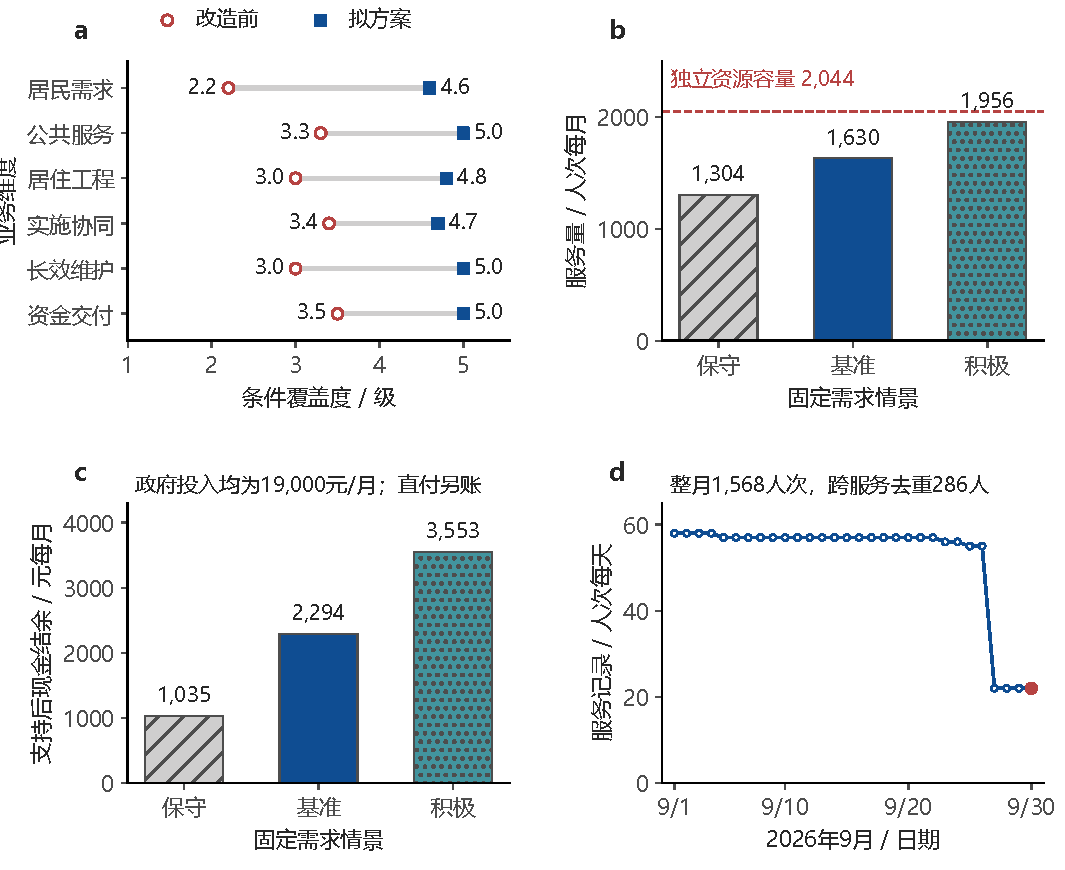
\includegraphics[width=\linewidth]{docs/figures/community-analysis-figure.pdf}
\caption{完整社区模拟数据的四项分析。a：六维现况与拟方案使用同一条件覆盖规则；b：固定需求情景的服务量与2044人次月容量；c：三种情景的支持后运营现金结余，政府直付维护另账；d：1568条模拟台账的逐日服务量。各面板由归档数据直接生成，不包含真实运营效果或统计置信区间。}
\end{figure}

\clearpage
\section{计算机制与情景检验细节}\label{app:science}
本附录保留容量约束、收支切换、参数敏感性及经济情景的计算细节。正文的财务与社会收益比较复用这些计算入口；具体演示值用于检查公式和展示方案变化。
\subsection{操作自测口径与原始计时}

2026年10月15日，在服务已启动、两份求是村原文已归档并完成解析的条件下，固定两个问题及五项核对标准：供水楼幢、252户范围、留博楼排除原因、报道时点的进场阶段、加梯征求意见阶段。Codex分别执行逐份查看与工作台检索两条自动浏览器路径，五项均可回到原文核对。计时从路径操作开始至读取对应内容结束，资料获取、导入及人工被试时间不在计时范围。

逐份查看路径耗时8.851秒；工作台路径耗时39.389秒，包含一次对未登记举措筛选条件的纠正。另行测得两次本地检索接口响应为29.777与19.498毫秒，合计49.275毫秒，前五条结果找回三处预先登记的目标片段（3/3）。自动操作耗时与接口响应分别记录；本次为单项目操作自测，未开展人工被试实验，不由接口毫秒数或两条自动路径推算人工节时率。完整问题、范围、返回定位、计时及操作条件见\path{research/test_results/decision-value-selftest-20261015.json}。

\subsection{用分时容量纠正月度合计的乐观假设}

服务需求具有时段差异，月平均量会掩盖高峰时段的供给不足。\cite{green2007} 在预约无法改期、服务不能跨时段结转的假设下，设第$t$时段需求为$D_t$、有效容量为$K_t$，则
\begin{equation}
 V=\sum_t\min(D_t,K_t),\qquad
 U=\frac{V}{\sum_tK_t},\qquad
 L=\sum_t\max(0,D_t-K_t).
\end{equation}
这里$V$为服务人次，$U$为容量利用率，$L$为未满足需求人次。由于
\begin{equation}
 \sum_t\min(D_t,K_t)\leq\min\!\left(\sum_tD_t,\sum_tK_t\right),
\end{equation}
月合计计算应被理解为需求可在容量间匹配时的上限。演示中两时段需求为80、20人次，容量各为50人次；分时结果为70人次、未满足30人次、利用率70\%，月合计上限则为100人次。系统同时显示两种结果及30人次的高估量。

界面已支持逐时段输入需求、场次、每场容量及其依据；启用后按分时记录计算。一个时段类别内部仍需说明需求能够匹配该类场次。当前保留独立资源检查，共用场地需要先明确分配；研究并未引入未经校准的随机排队或预约改期模型。

\subsection{用收支切换值说明结论离边界有多远}

Green Book将敏感性分析与切换值用于识别改变方案判断的关键条件。\cite{greenbook2026} 月度运营核算先区分运营方现金与财政支付。设服务人次为$V$、收费比例为$q$、每收费人次价格为$p$、每人次变动成本为$v$、固定运营支出为$F$，其他经营收入为$R_o$、政府购买服务为$G_p$、运营补贴为$S$、其他支持为$H$，则
\begin{equation}
 \Pi=V(qp-v)+R_o+G_p+S+H-F.
\end{equation}
政府直接支付的其他运营费用另列，不重复进入运营方支出；财政支出按政府购买服务、补贴和政府直接支付汇总。建设投资、贷款本息和折旧沿用建设经济模型。

对单一服务，保持价格、收费比例、单位变动成本及其他收支不变，且$qp-v>0$时，保本人次为
\begin{equation}
 V^*=\left\lceil\frac{\max(0,F-R_o-G_p-S-H)}{qp-v}\right\rceil.
\end{equation}
程序同时核对$V^*$是否超过登记容量；在当前服务量保持不变的条件下，另算最低收费和最低收费比例。若收费比例阈值超过1、所需人次超过容量或关键分母为0，直接显示对应条件，而不以总分抵消。

基准演示设月容量520人次、需求400人次、收费比例40\%、每收费人次10元、每服务人次变动成本2元、固定支出10000元、其他经营收入1000元、政府购买服务2000元和补贴6000元。按同一正式计算函数得到：
\begin{center}\small
\begin{tabular}{@{}L{55mm}rL{70mm}@{}}
\toprule 指标 & 结果 & 对判断的具体影响\\\midrule

运营现金结余 & -200元/月 & 基准输入仍有现金缺口\\
按当前服务量所需补贴 & 6200元/月 & 比演示的6000元补贴多200元\\
保本人次 & 500人次/月 & 达到容量的96.15\%，仍需取得相应需求\\
保持400人次时最低收费 & 11.25元/收费人次 & 固定需求的切换值；调价后的需求需另估计\\
保持400人次时最低收费比例 & 45\% & 保持10元收费和其他条件不变\\

\bottomrule\end{tabular}\end{center}
登记容量满负荷时，现金结余只有40元/月；固定支出增至11000元时，保本需要1000人次，超过520人次容量。这比仅展示“积极情景不亏损”更具体地指出了需要核实的固定费用、需求及补贴条件。

\begin{figure}[htbp]
\centering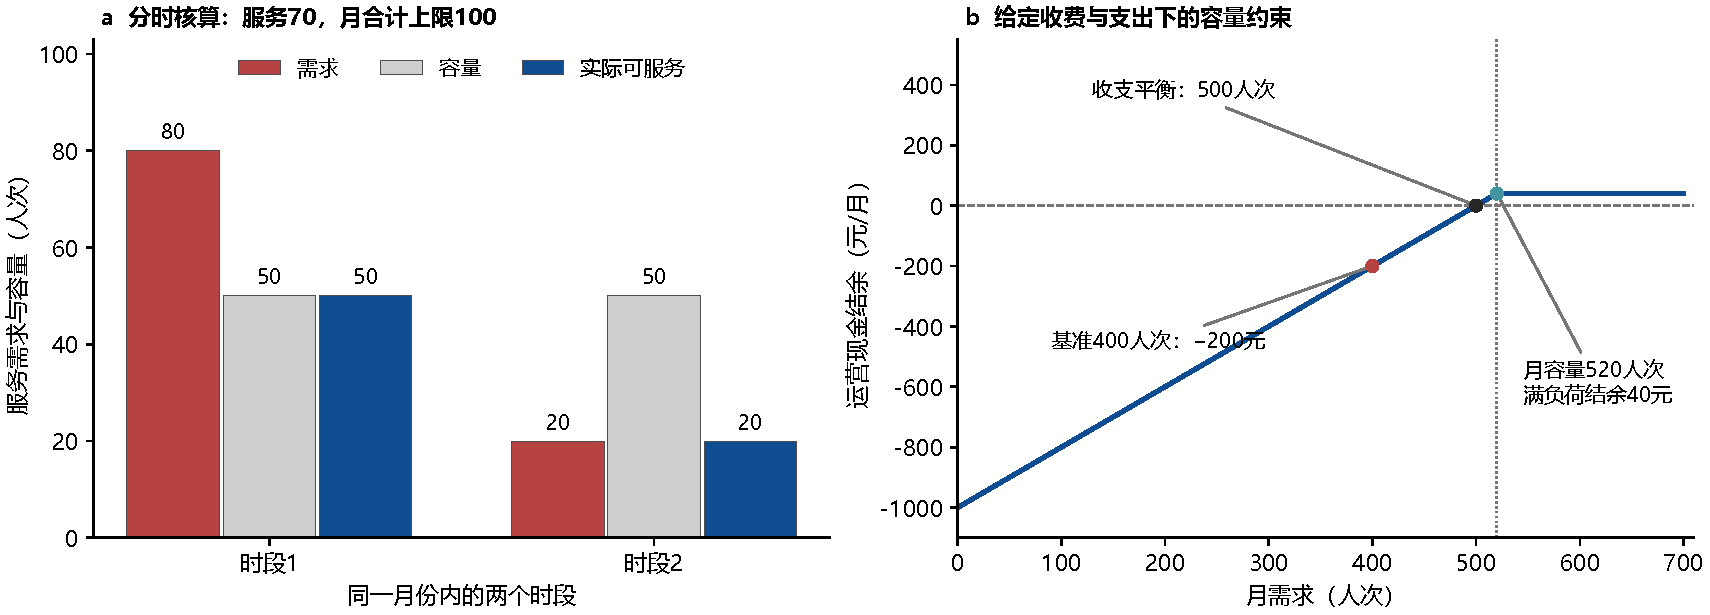
\includegraphics[width=\linewidth]{docs/figures/operations-scientific-checks.pdf}
\caption{同一核算函数的机制检验。a为不可跨时段结转的容量例子；b为给定收费、支出与补贴下的月度需求压力测试。全部为明确标注的演示输入，图中现金边界与表中阈值来自同一结果记录。}
\label{fig:scientific-operations}
\end{figure}

\subsection{把参数范围、单参影响和组合结果一起保存}

系统增加逐参数的下界、基准、上界、范围来源、取得日期及适用说明。单参数分析每次只改一个输入，并调用同一核算函数；组合分析枚举最多6个参数的端点组合。来源不明的百分比不能作为经验分布。\cite{gao2020} 本轮演示以需求倍率0.7至1.3、固定支出9000至11000元测试计算机制，范围性质明确标为人工压力设定。

\begin{center}\small
\begin{tabular}{@{}L{49mm}rrrr@{}}
\toprule 改变的参数 & 下界结余 & 基准结余 & 上界结余 & 结余跨度\\\midrule

固定支出：月度现金事项 & 800 & -200 & -1200 & 2000\\
活动服务：服务需求倍率 & -440 & -200 & 40 & 480\\
\bottomrule\end{tabular}\end{center}
结余及跨度单位均为元/月。四个参数端点组合得到的现金结余为-1440至1040元/月，最大缺口为1440元/月。固定支出的单参跨度为2000元，大于需求变化的480元；在这组演示范围内，固定费用依据更值得优先补充。

这些输出称为“已测试参数组合范围”。若要估计亏损概率或概率覆盖区间，还需有输入分布与依赖关系的依据。JCGM 101要求先依据知识指定输入分布或联合分布，再进行传播计算。\cite{jcgm2008} 本轮不以任意均匀或三角分布把压力测试包装成真实风险概率。

\subsection{两组演示与一个缺项分支}

经济示例采用五年、5\%折现率的演示假设：
\begin{center}\small
\begin{tabular}{lrrl}\toprule
\textbf{模式组合} & \textbf{经营NPV 元} & \textbf{峰值缺口 元} & \textbf{计算状态}\\\midrule
保留整治＋服务运营 & 56,392.31 & 0 & 可开展专项调查\\
部分保留＋局部拆建＋经营 & -285,683.11 & 1,000,000 & 展示调整因素\\
整体拆建，权利与价格缺项 & 空值 & 空值 & 补关键资料\\\bottomrule
\end{tabular}\end{center}

第一方案的保本月租为115.18元/平方米/月。程序保留出资、贷款、收入和业主资产效益的独立账，展示哪些参数使收益或资金缺口变化。这组示例的数据标签均为演示假设。

适老示例采用演示住区1000人、老年占比33\%、目标群体330人；按同一随机序列比较基线与改善，结果如下：
\begin{center}\small
\begin{tabular}{llrrrr}
\hline
组合 & 采用情景 & 可达人数 & 使用人数 & 覆盖率(\%) & 容量使用率(\%) \\
\hline
基线组合 & 低 & 110 & 45 & 13.64 & 28.33 \\
基线组合 & 中 & 110 & 72 & 21.82 & 46.67 \\
基线组合 & 高 & 110 & 91 & 27.58 & 62.22 \\
改善组合 & 低 & 330 & 143 & 43.33 & 53.1 \\
改善组合 & 中 & 330 & 213 & 64.55 & 81.67 \\
改善组合 & 高 & 330 & 235 & 71.21 & 94.05 \\
\hline
\end{tabular}
\end{center}

中采用情景下，去重使用人数由72人增加到213人，增加141人；使用人群覆盖率提高42.73个百分点，月访问量由336次增加到1372次。这是给定人口、路线、设施和采用参数后的预测结果，后续用台账和实际使用记录校准。

演示另保留关键权利、价格或容量字段空值，输出\textbf{“先补充关键资料再判断”}，并显示影响的指标和补填任务。默认缺省的非核心字段只影响其对应规则，其他有完整输入的事项继续运行。

\subsection{用冻结预测和独立对象核验，而非用演示自证准确}

当前应用可冻结预测输入、计算版本、证据和时间，再登记同一中心完整月份的原始台账，保存实际减预测的误差和绝对误差。实际值为0时不计算百分比误差。目标月开始前冻结才归入前瞻对照；事后重建只作历史回放。

后续跨社区检验按社区分组，同一社区的居民记录不能随机拆入训练与测试两侧；跨期检验以较早月份校准、较晚月份验证。数据清理、参数确定和阈值选择只使用校准部分。\cite{groupcv} 本轮已将真实问卷审计、确定性机制检验和月度实绩接口分别实现，实际运营台账尚待取得。

措施展示也采用明确计数单位：项目、案例/规则性质及措施类别相同的记录形成一个默认折叠的措施组，展开后保留不同楼栋、阶段、来源和原卡。宽泛类别中不同原文名称仍可逐项查看。重复提取同一项目、同一来源版本、完全相同字段的记录时复用原卡，不重置复核状态；不同金额、对象或阶段继续分别保存。由此避免把多个原文片段或重复提取误当作多个独立案例。

\subsection{程序应用与复现入口}

现有项目工作台已接入分时录入、收支切换值、带范围依据的敏感性和组合结果；历史工程库支持按面积口径及价格年筛选、显示同口径参考组和排除原因。报告导出保留来源、固定条件、缺项及计算结果，原冻结版本按原值回读。

技术核验分三层：公式与边界测试检查容量守恒、分母和费用重复；HTTP与界面检查录入、保存、读回与导出；真实决策效果留待实际运营台账和独立项目评测。复现采用同一计算入口，表格和图形读取生成结果，关键源文件如下：
\begin{itemize}
\item 月度计算与科学核验：\path{services/capabilities/community_operations.py}、\path{services/capabilities/operations_science.py}。
\item 演示结果复现：\path{scripts/build-scientific-methods-evidence.py}；造价分组复现：\path{scripts/verify-expanded-cost-library.ts}。
\item 用户表接收：\path{scripts/intake-historical-projects-workbook.py}；公开问卷审计：\path{scripts/audit-hangzhou-survey.py}。
\end{itemize}


\begin{thebibliography}{99}
\small
\setlength{\itemsep}{1pt}
\setlength{\parsep}{0pt}
\setlength{\parskip}{0pt}
\bibitem{water} 浙江在线. 浙大求是社区推进二次供水改造. 2023年8月18日. \href{https://town.zjol.com.cn/czjsb/202308/t20230818_26113017.shtml}{原文链接}.
\bibitem{trust} 浙江日报，杭州网转载. 西湖区三方协同为居民幸福加码. 2023年12月28日. \href{https://hznews.hangzhou.com.cn/shehui/content/2023-12/28/content_8666802.htm}{原文链接}.
\bibitem{neighbor} 西湖报. 这个康养生活综合体已焕新启用. 2025年10月28日. \href{https://xhb.xihunet.cn/h5/html5/2025-10/28/content_9248_18995526.htm}{原文链接}.
\bibitem{cuiyuan} 浙江在线. 翠苑一区老旧小区改造工程顺利竣工. 2022年10月26日. \href{https://cs.zjol.com.cn/kzl/202210/t20221026_24968653.shtml}{原文链接}.
\bibitem{paper} Renovation priorities for old residential districts based on resident satisfaction: An application of asymmetric impact-performance analysis in Xi'an, China. PLOS ONE, 2021. DOI: \href{https://doi.org/10.1371/journal.pone.0254372}{10.1371/journal.pone.0254372}.
\bibitem{policy} 国务院办公厅. 关于全面推进城镇老旧小区改造工作的指导意见. 国办发〔2020〕23号，2020年7月10日. \href{https://www.ndrc.gov.cn/fzggw/jgsj/tzs/sjdt/202007/t20200728_1234742.html}{国家发展改革委公开全文}.
\bibitem{elevator} 杭州市西湖区灵隐街道. 浙大求是社区求是村75幢1单元加装电梯征求意见公告. 2024年9月18日. \href{https://www.hzxh.gov.cn/art/2024/9/18/art_1229516984_59041263.html}{原文链接}.
\bibitem{renewal2025} 中共中央办公厅、国务院办公厅. 关于持续推进城市更新行动的意见. 2025年5月2日. \href{https://www.mee.gov.cn/zcwj/zyygwj/202505/t20250516_1119546.shtml}{官方全文}.
\bibitem{hzmode} 杭州市人民政府办公厅. 全面推进城镇老旧小区改造工作的实施意见. 杭政办函〔2022〕10号，2022年2月14日. \href{https://zfgb.hangzhou.gov.cn/10/105220253/t117220253054/518761.shtml}{杭州公报全文}.
\bibitem{ndrcfinance} 国家发展改革委. 企业投资项目可行性研究报告编写参考大纲 2023年版. 第六部分. \href{https://www.ndrc.gov.cn/xxgk/zcfb/ghxwj/202304/P020230407401908613786.pdf}{官方PDF}.
\bibitem{zhegongdata} 杭州政协网转载杭州日报. 浙工新村自主更新预算报道. 2024年1月19日. \href{https://www.hzzx.gov.cn/cshz/content/2024-01/19/content_8677402.htm}{原文链接}.
\bibitem{zhegongfollow} 上观新闻. 浙工新村自主更新回访. 2026年8月19日. \href{https://www.jfdaily.com/wx/detail.do?id=1162310}{回访原文}.
\bibitem{shmix} 上海市普陀区发展改革委. 曹杨八村75至76号旧住房成套改造项目批复. 2025年. \href{https://www.shpt.gov.cn/zhengwu/xmjyssp-fgwzdgz/2025/42/194395.html}{批复全文}.
\bibitem{gao2020} U.S. Government Accountability Office. Cost Estimating and Assessment Guide: Best Practices for Developing and Managing Program Costs. GAO-20-195G, 2020, pp.93--98, 134--137, 164, 180. \href{https://www.gao.gov/assets/gao-20-195g.pdf}{官方指南}.
\bibitem{greenbook2026} HM Treasury. The Green Book (2026). 2026年2月5日版，Sensitivity analysis and switching values; Economic transfers. \href{https://www.gov.uk/government/publications/the-green-book--2/the-green-book-2026}{官方正文}.
\bibitem{mca2009} Communities and Local Government. Multi-criteria analysis: a manual. 2009. \href{https://www.gov.uk/government/publications/multi-criteria-analysis-manual-for-making-government-policy}{英国政府方法手册}.
\bibitem{mcda2024} HM Treasury. Use of Multi-Criteria Decision Analysis in options appraisal of economic cases. 2024年5月16日更新，第4.4至4.5节：摆幅赋权与敏感性。\href{https://www.gov.uk/government/publications/green-book-supplementary-guidance-multi-criteria-decision-analysis/use-of-multi-criteria-decision-analysis-in-options-appraisal-of-economic-cases}{官方方法指导}.
\bibitem{green2007} Green L V, Kolesar P J, Whitt W. Coping with Time-Varying Demand When Setting Staffing Requirements for a Service System. Production and Operations Management, 2007, 16(1):13--39. DOI: \href{https://doi.org/10.1111/j.1937-5956.2007.tb00164.x}{10.1111/j.1937-5956.2007.tb00164.x}.
\bibitem{jcgm2008} JCGM. Evaluation of measurement data---Supplement 1 to the GUM---Propagation of distributions using a Monte Carlo method. JCGM 101:2008, Section 5. \href{https://www.bipm.org/documents/20126/2071204/JCGM_101_2008_E.pdf}{BIPM官方全文}.
\bibitem{hangzhou2026} Sun Y, Hu W, Xia X. How self-governance willingness and participation efficacy shape residents' satisfaction with urban public services: Evidence from neighborhood renewal in Hangzhou, China. PLOS ONE, 2026, 21(1):e0341177. \href{https://doi.org/10.1371/journal.pone.0341177}{正文与原始附件}.
\bibitem{cdcvariance} CDC, National Center for Health Statistics. NHANES Tutorials: Variance Estimation. \href{https://wwwn.cdc.gov/nchs/nhanes/tutorials/varianceestimation.aspx}{复杂抽样方差说明}，访问日期2026年10月13日.
\bibitem{nistwilson} NIST/SEMATECH. e-Handbook of Statistical Methods: Confidence intervals for a binomial proportion. \href{https://itl.nist.gov/div898/handbook/prc/section2/prc241.htm}{比例区间公式}，访问日期2026年10月13日.
\bibitem{groupcv} scikit-learn developers. Cross-validation: evaluating estimator performance. Group and time-series cross-validation. \href{https://scikit-learn.org/stable/modules/cross_validation.html}{官方方法说明}，访问日期2026年10月13日.
\bibitem{gzyouth} 广州公共资源交易中心. 夏港街青年苑老旧小区改造项目施工总承包合同公示. 签约日期2024年9月2日. \href{https://ywtb.gzggzy.cn/jyfw/002001/002001001/20240904/0020010011010131.html}{官方原文}.
\bibitem{gzhong} 广州公共资源交易中心. 夏港街鸿中楼老旧小区改造项目施工合同公示. 签约日期2024年9月27日. \href{https://ywtb.gzggzy.cn/jyfw/002001/002001001/20241011/0020010011015508.html}{官方原文}.
\bibitem{shcang} 上海市住宅修缮工程交易平台. 江川路街道沧源二村美丽家园综合修缮项目施工中标结果. 中标日期2026年8月29日. \href{https://xsjypt.fgj.sh.gov.cn/cebea-bid-result!view.do?packageId=5fcd587e-411f-4617-9112-cf75a4b99372}{官方原文}.
\bibitem{shsea} 上海市住宅修缮工程交易平台. 七宝镇海上新村美丽家园综合修缮项目施工中标结果. 中标日期2026年8月28日. \href{https://xsjypt.fgj.sh.gov.cn/cebea-bid-result!view.do?packageId=edc6719e-876e-4613-9879-e03a5cc8084d}{官方原文}.
\bibitem{psobp2026} 王宝龙，王杰，刘广杰. PSO--BP神经网络模型在改造工程造价预测的应用研究：以广东省为例. 工程管理学报，2026，40(3):138--145. DOI: \href{https://doi.org/10.13991/j.cnki.jem.2026.03.022}{10.13991/j.cnki.jem.2026.03.022}. 本次核对用户提供的8页PDF原件.
\bibitem{nestedcv} scikit-learn developers. Nested versus non-nested cross-validation. \href{https://scikit-learn.org/stable/auto_examples/model_selection/plot_nested_cross_validation_iris.html}{官方方法示例}，访问日期2026年10月14日.
\bibitem{adam} Kingma D P, Ba J. Adam: A Method for Stochastic Optimization. ICLR, 2015. \href{https://arxiv.org/abs/1412.6980}{作者论文}.
\end{thebibliography}
\end{document}
